% !TEX root = ../dkilleffer-thesis-proposal.tex
%
\chapter{Prior Work}
\label{sec:priorwork}

\cleanchapterquote{A picture is worth a thousand words. An interface is worth a thousand pictures.}{Ben Shneiderman}{(Professor for Computer Science)}

%\Blindtext[2][1]

The idea of annotating videos is not entirely new or novel, but such tools have not become commonplace in the same way that high quality image editing software and facial recognition algorithms have brought new dimensions to digital photography.  YouTube has empowered people to share their recordings with the world in new ways and given rise to entirely new forms of entertainment.  In the realm of education with the rise in online education and increasing pressure to make class lectures available to students both on-campus and remote, many classes are now recorded and distributed online, and there has been some scholarly research work done to enable students to annotate and share notes on classes.

Some prior scholarly works in the area of video annotation include:


\begin{enumerate}
\item \href{http://opinion.city}{OpinionCity}, by Daniel P. Coffey: danielpcoffey@gmail.com \\
\\ 
OpinionCity is a website that was created by Daniel P. Coffey for a Digital Media Capstone project at Harvard Extension School.  It is a tool for real-time group feedback on videos that have been uploaded to YouTube and allows for collaborative, time-code based annotation of videos as well as whole-video annotations.  Users may select a video to "upload" to OpinionCity where the video from YouTube will play in an embedded player, and then users can add comments to the video at specific timecodes or apply their remarks to the entire video.  Users can also invite others to join in and comment on the video as well. \\
\\

%\begin{center}

%	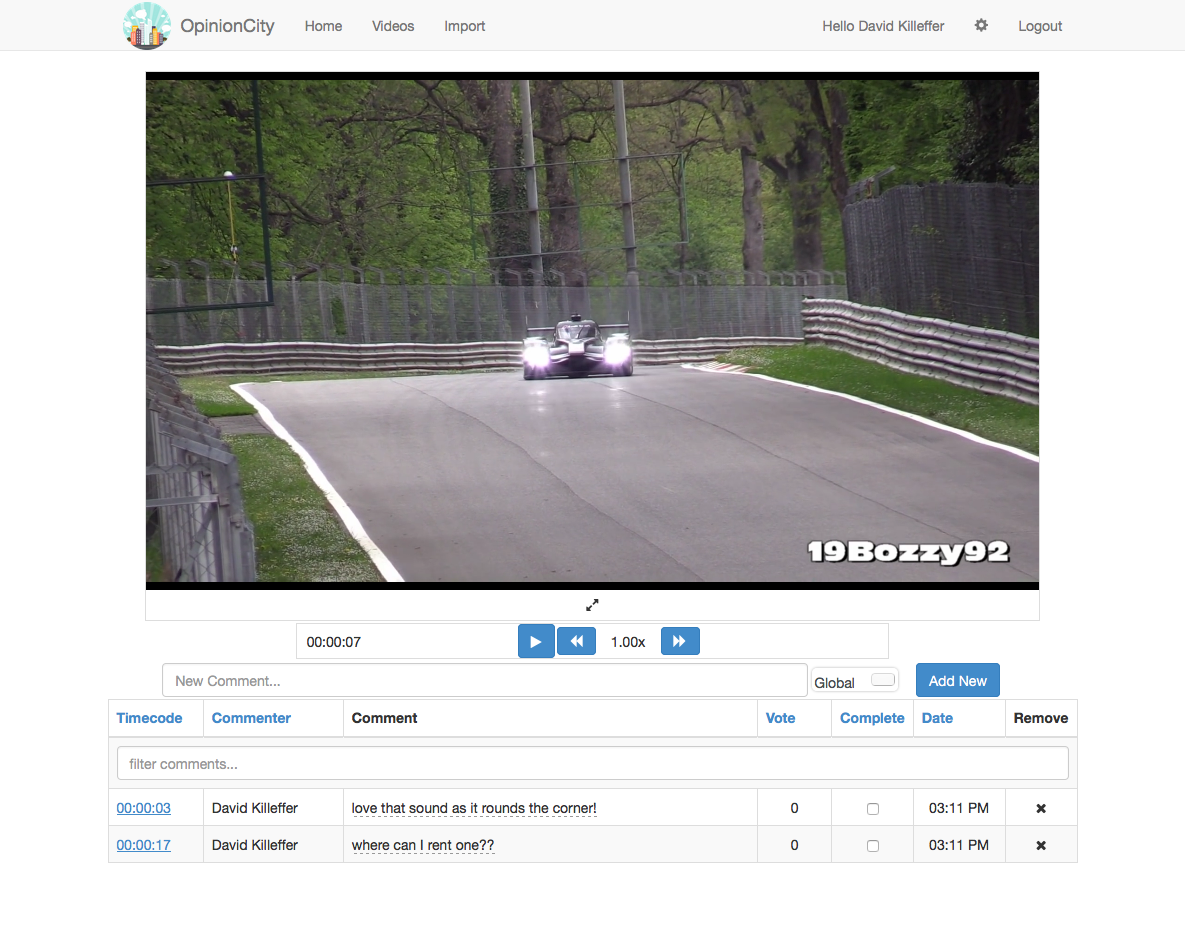
\includegraphics[width=6cm]{gfx/opinion-city/Screen Shot 2016-05-27 at 3.37.57 PM (2).png} \\[2mm]
%	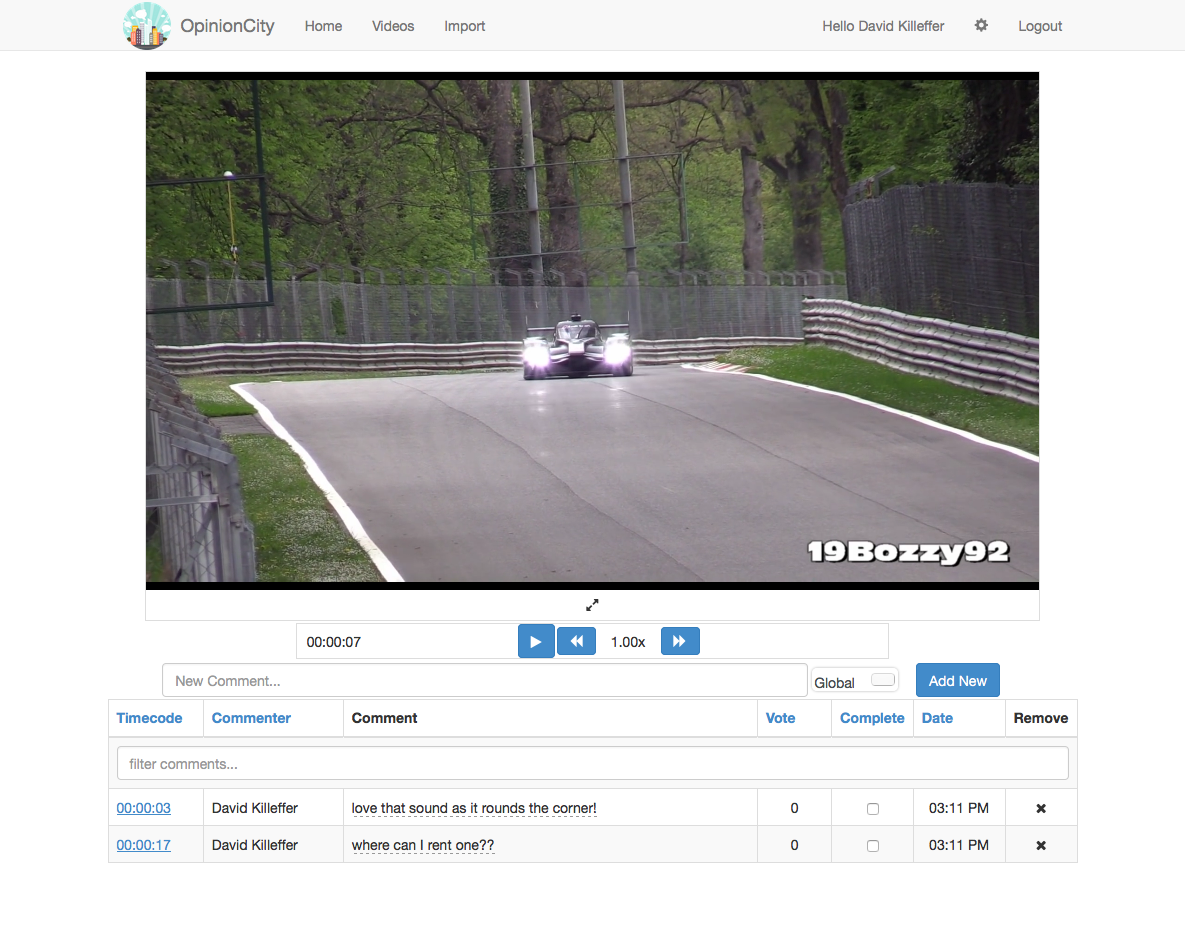
\includegraphics[width=6cm]{"gfx/opinion-city/Screen Shot 2016-05-27 at 3.37.57 PM (2).png"} \\[2mm]
%	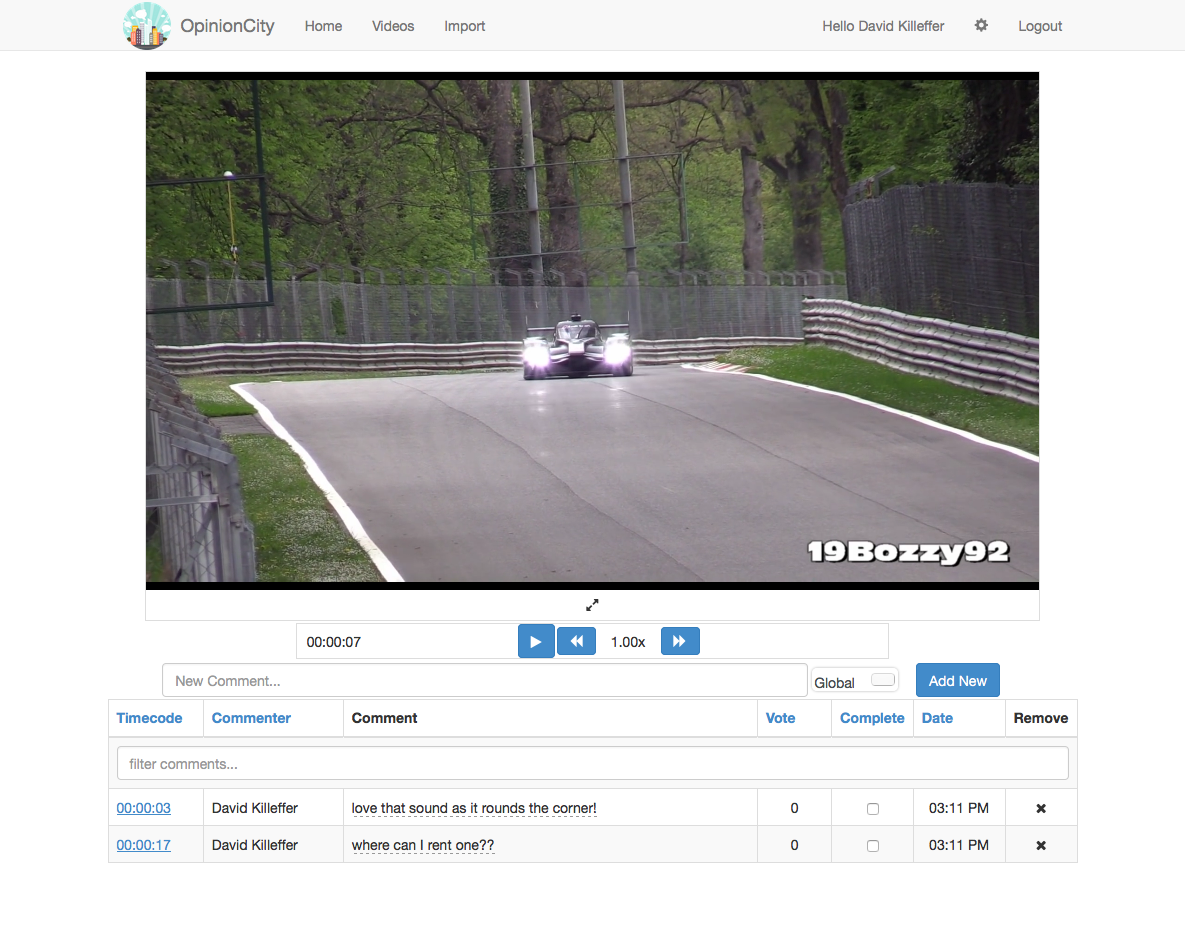
\includegraphics[width=6cm]{"gfx/opinion-city/car1.png"} \\[2mm]

	%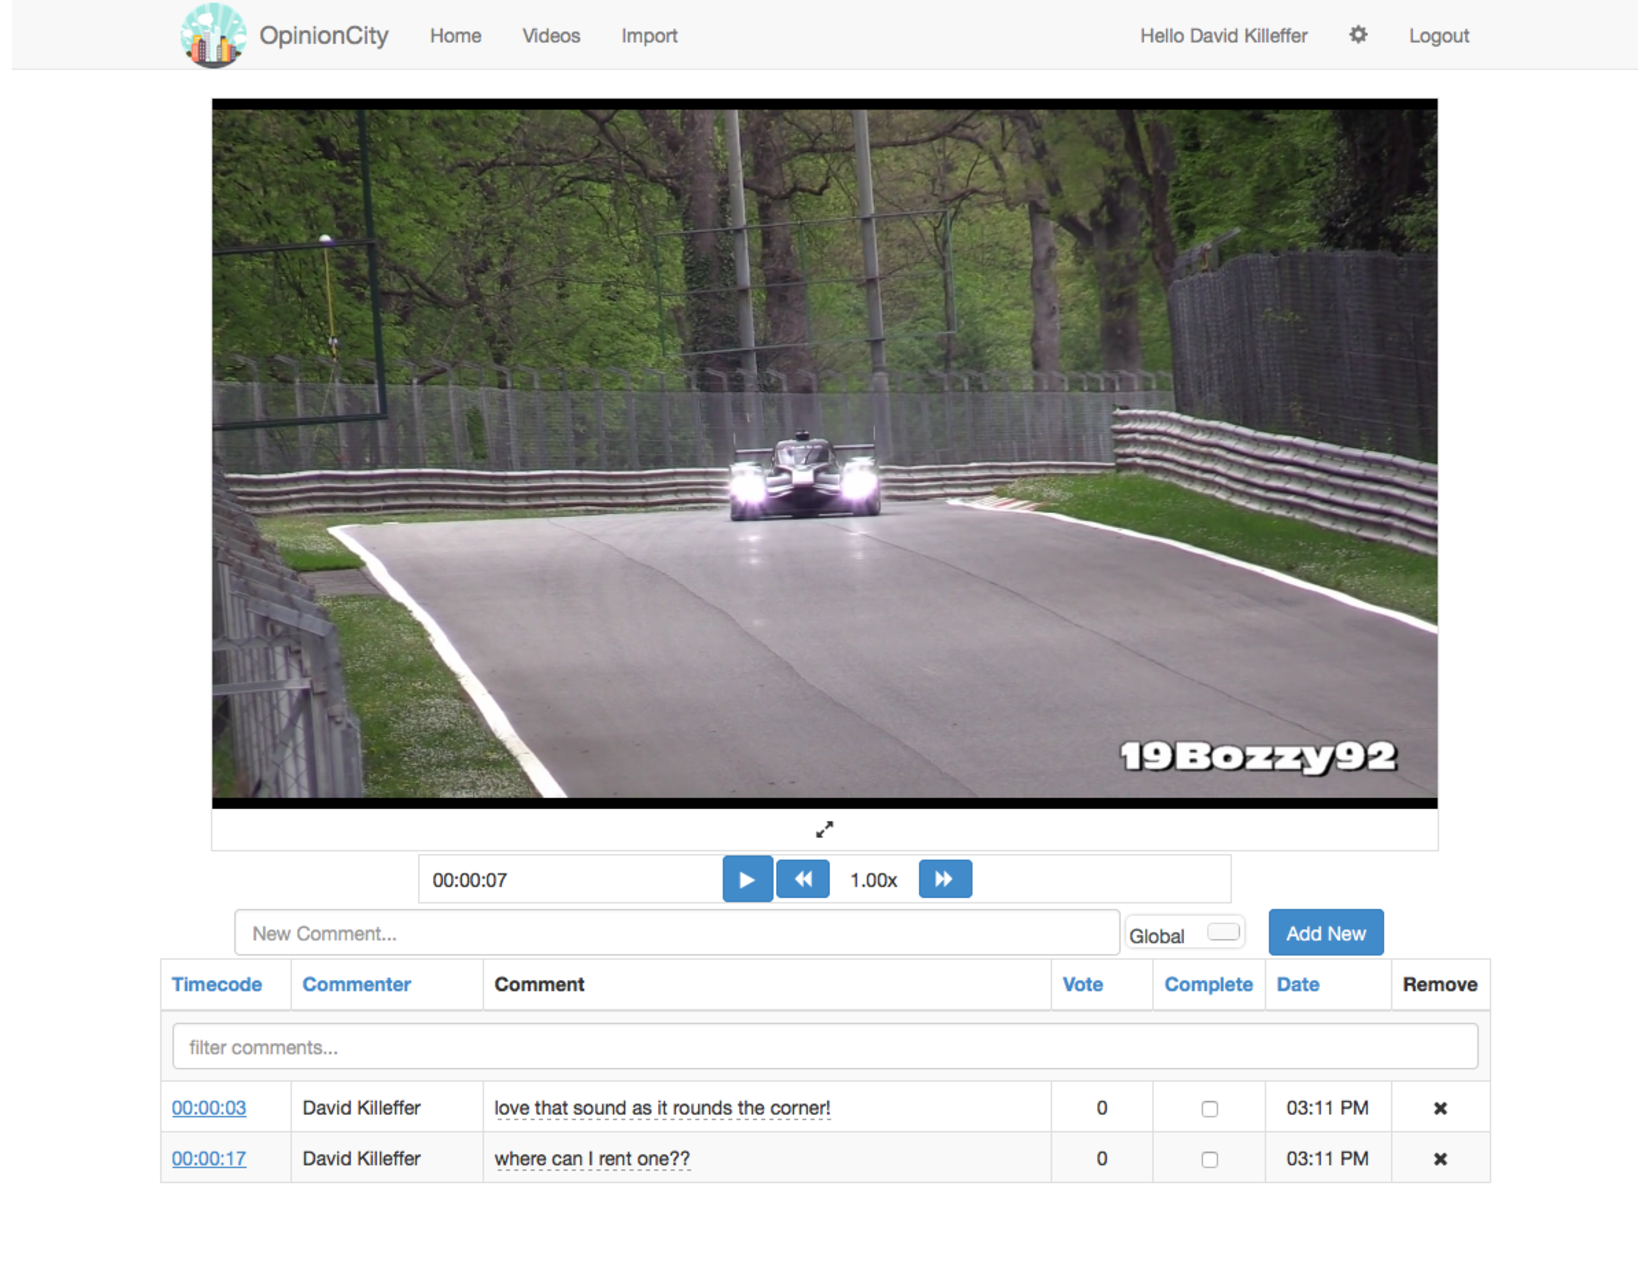
\includegraphics[width=18cm]{gfx/opinion-city/car1.pdf} \\[2mm]
	%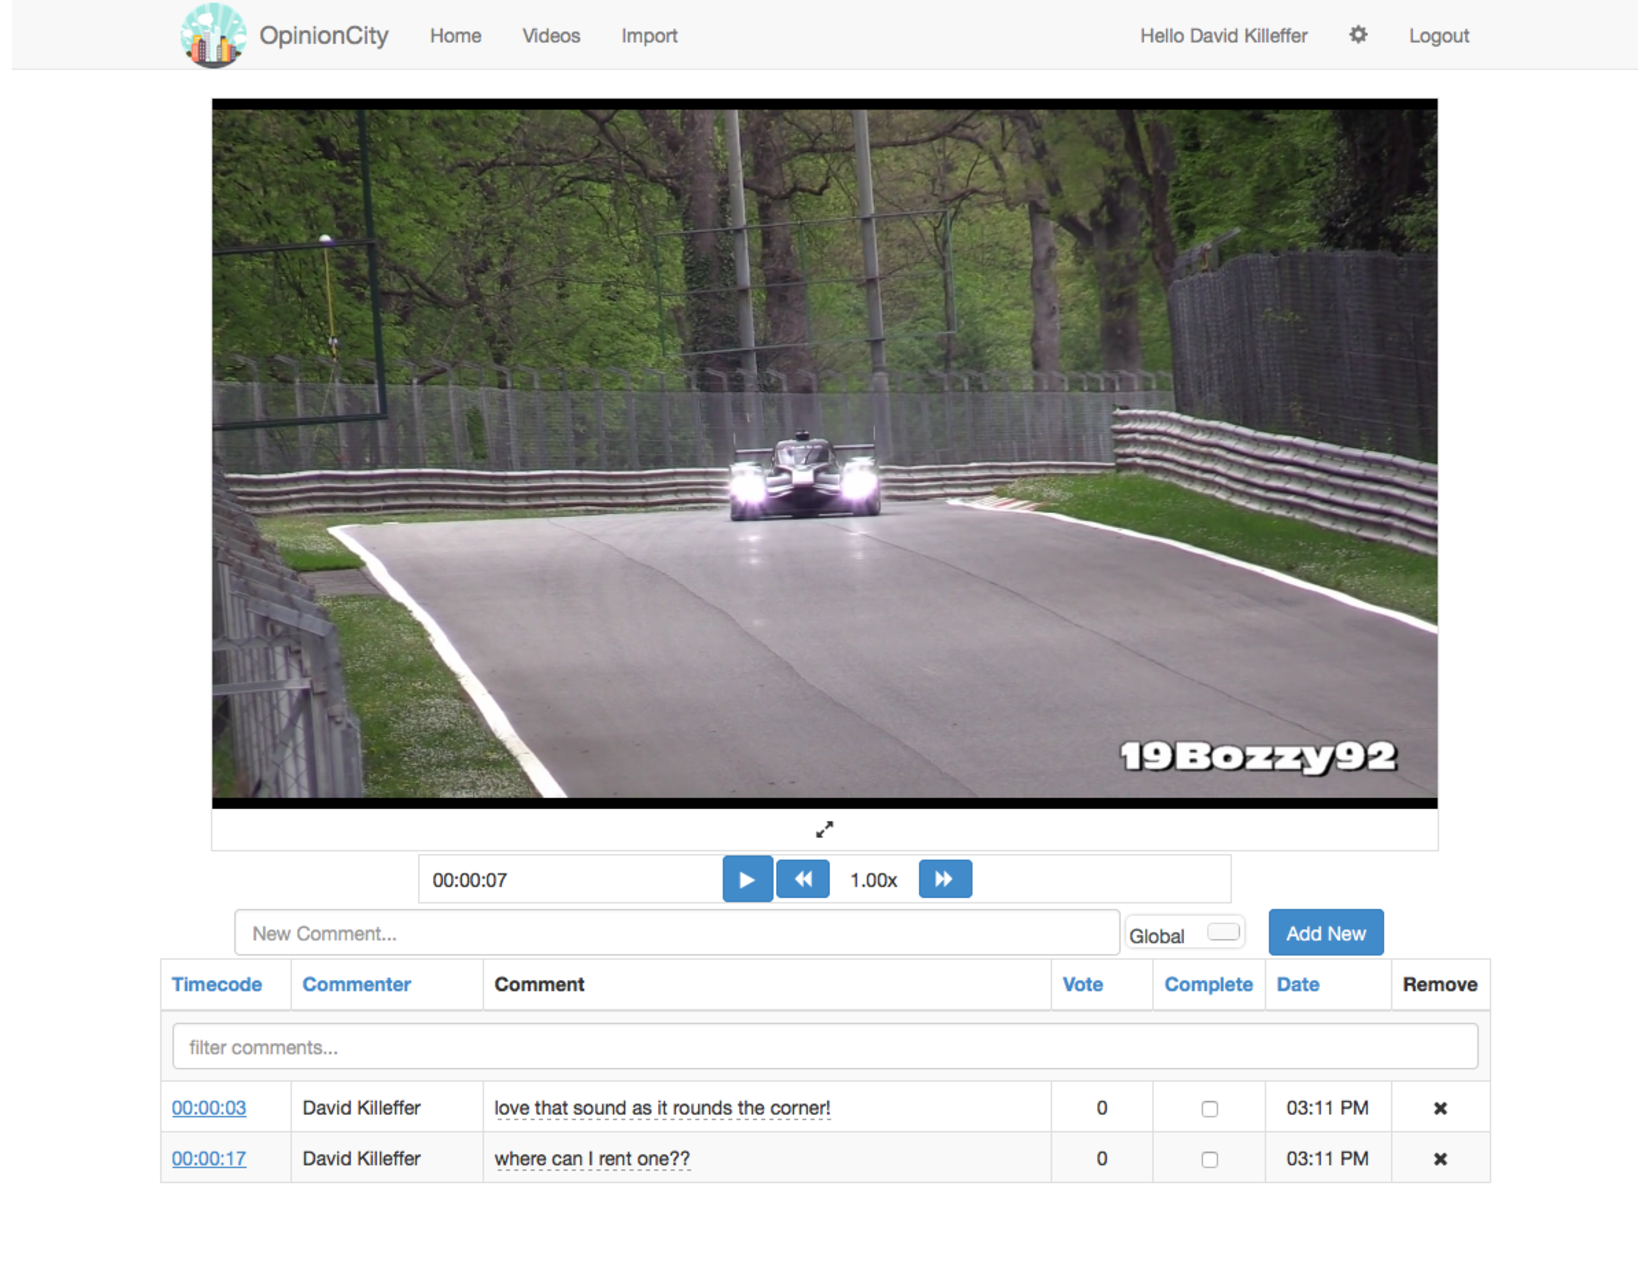
\includegraphics[scale=0.65]{gfx/opinion-city/car1.pdf} \\[2mm]
%	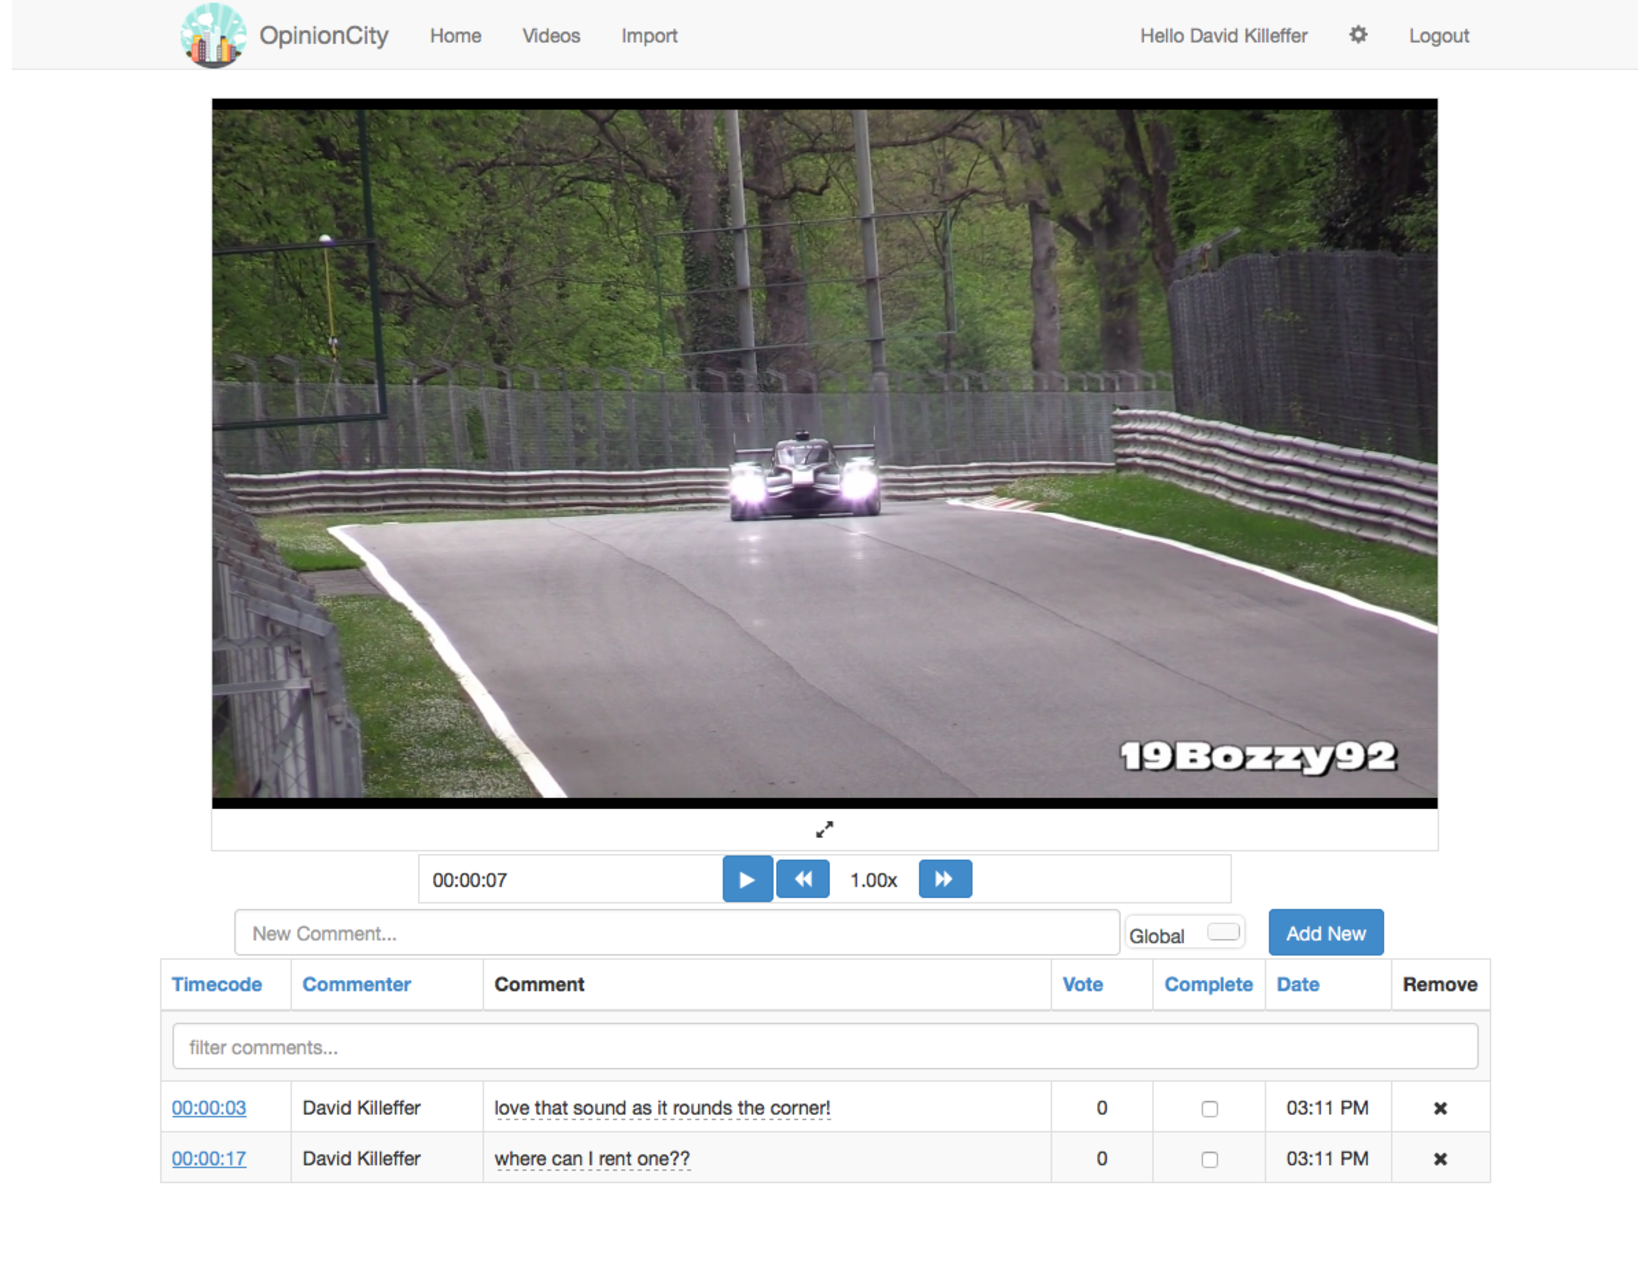
\includegraphics[scale=0.65]{gfx/opinion-city/car1.pdf} \\


%{\centering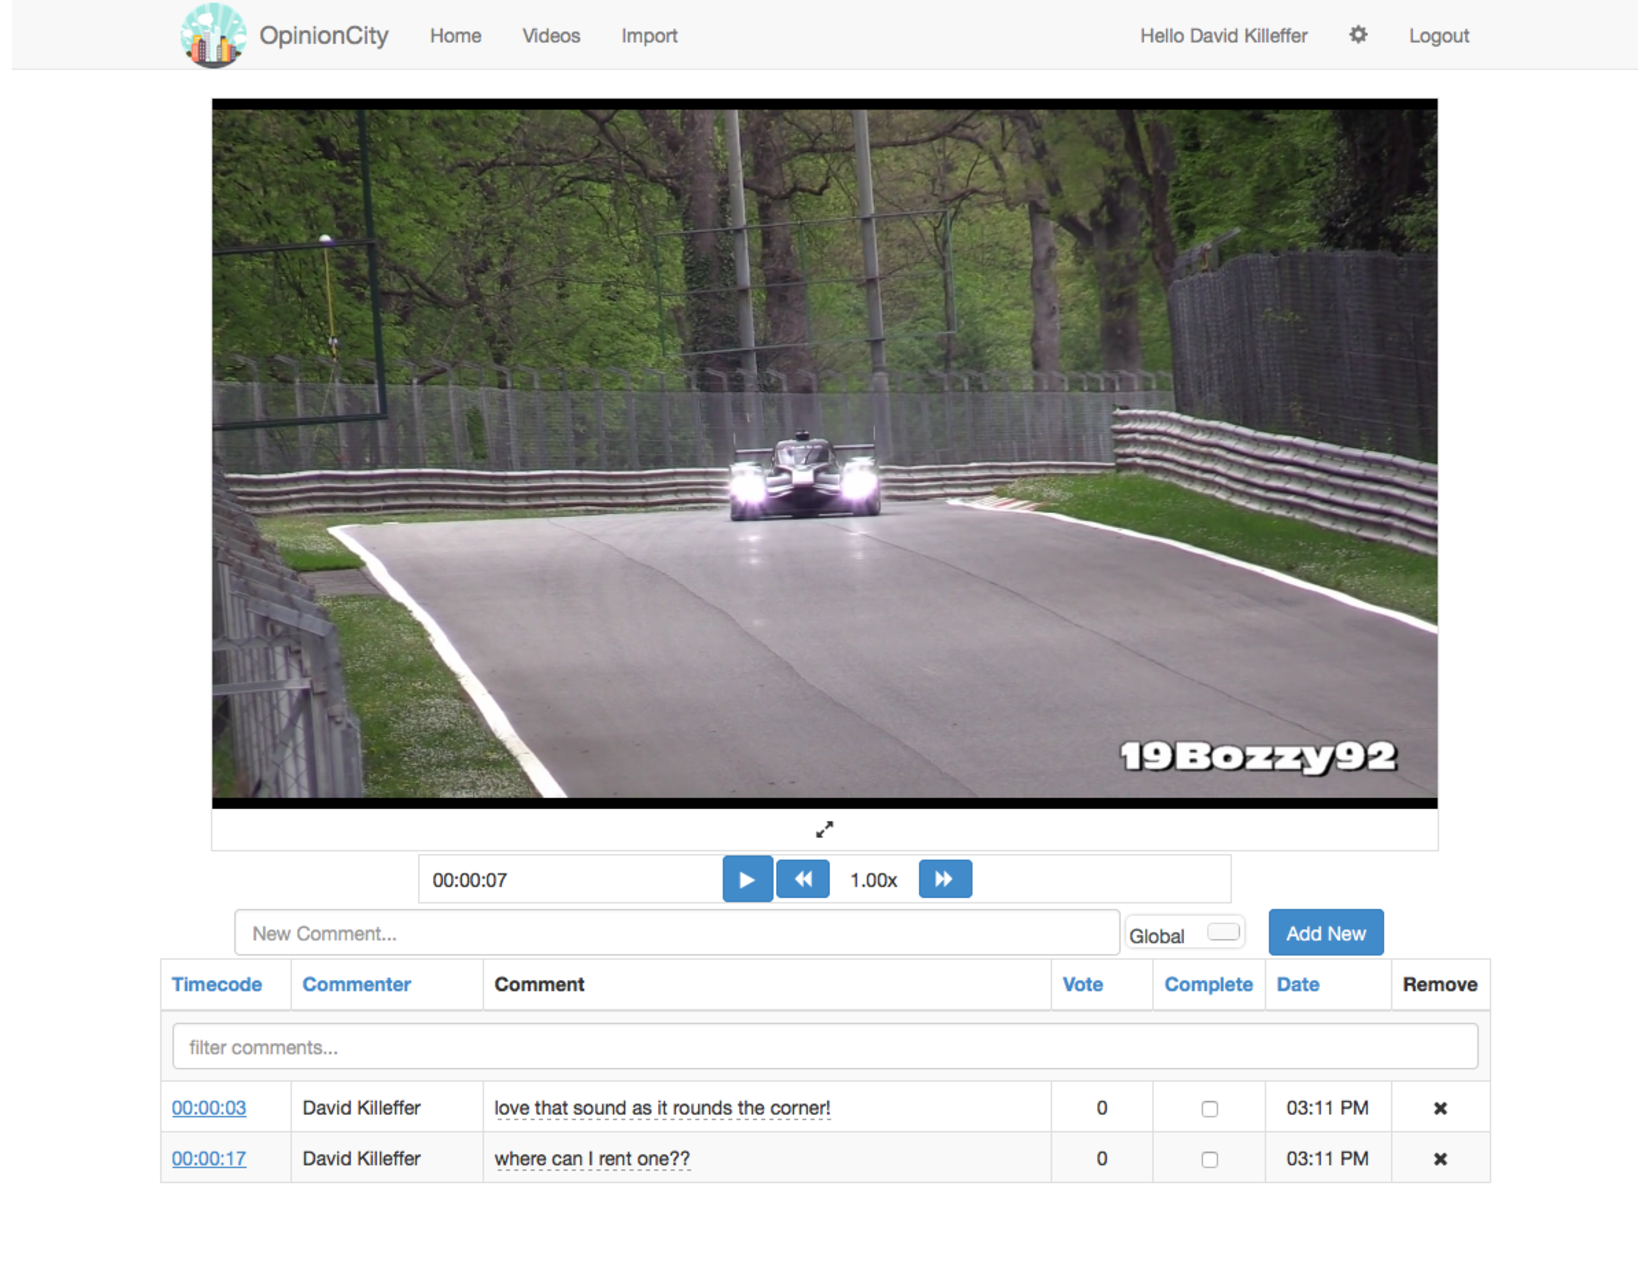
\includegraphics[scale=0.65]{gfx/opinion-city/car1.pdf}} \\
{\centering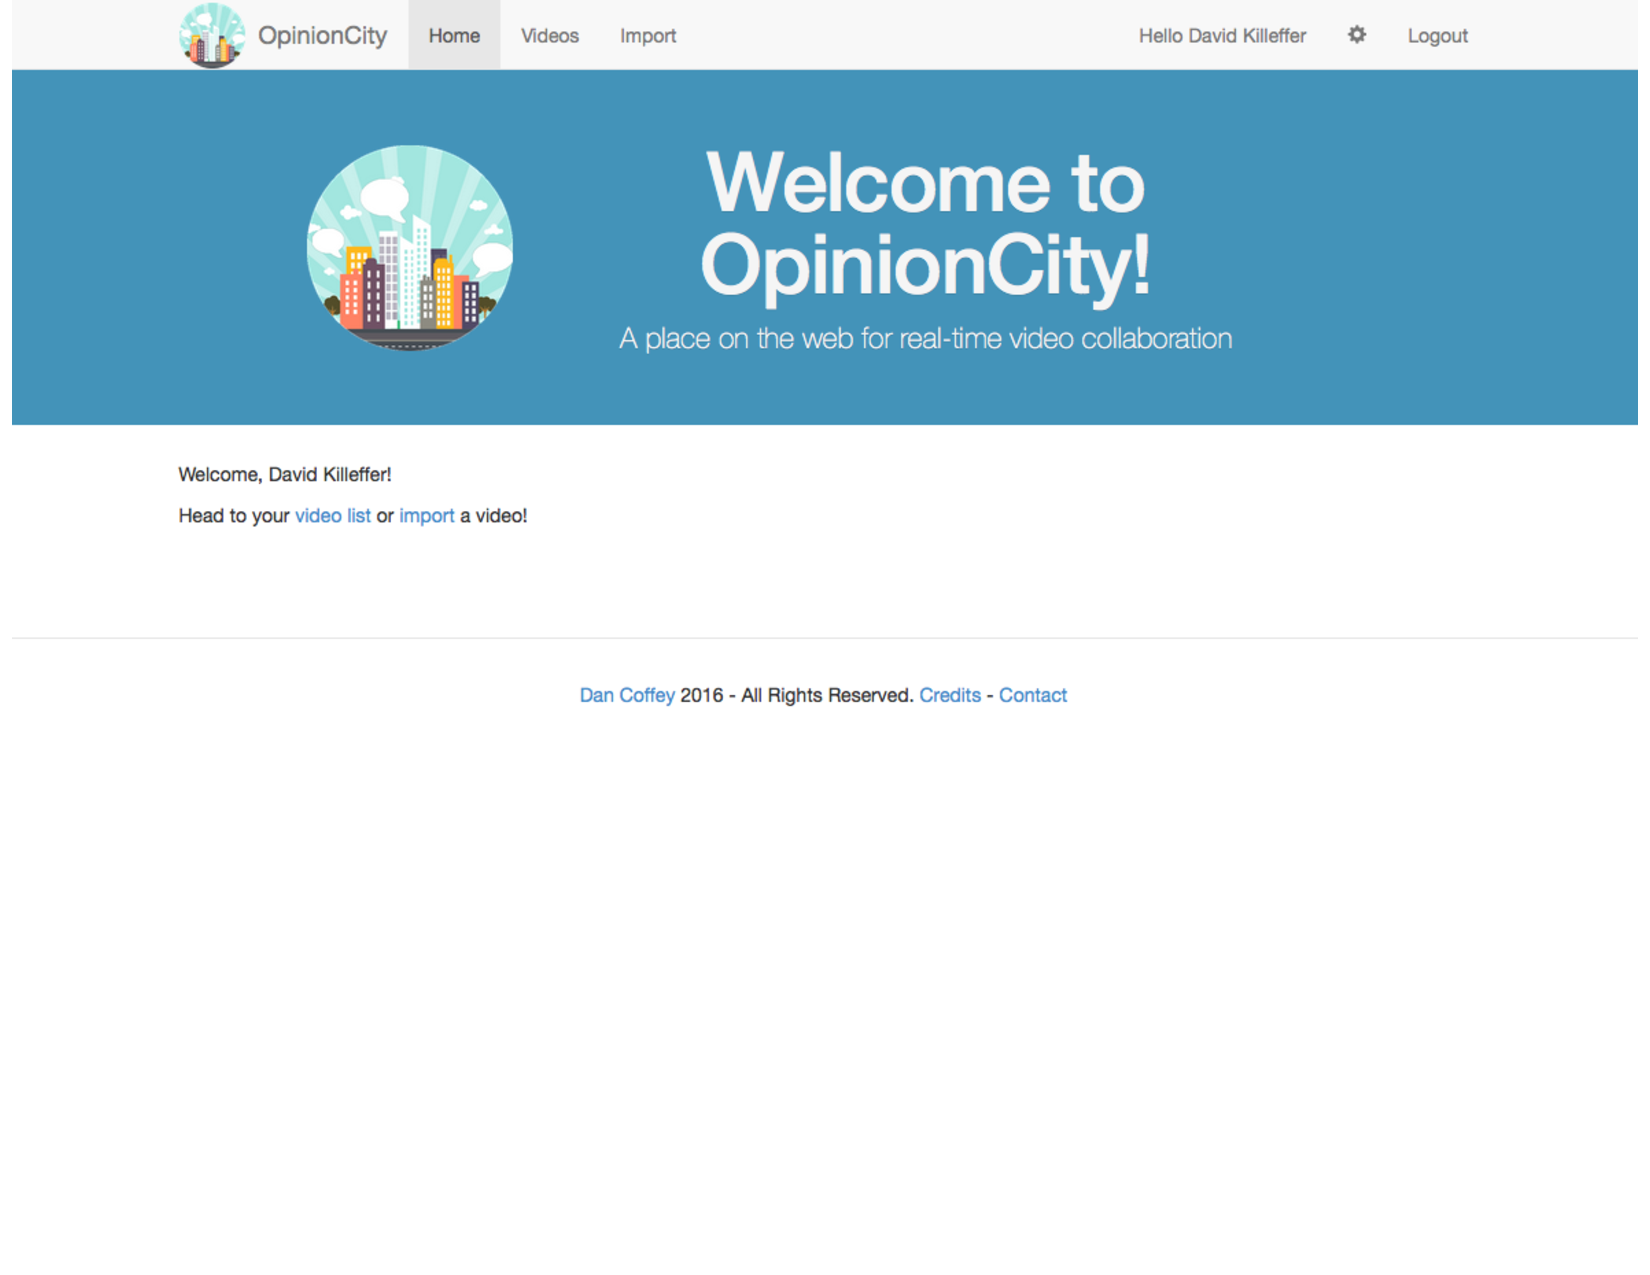
\includegraphics[width=1\textwidth]{gfx/opinion-city/homepage1.pdf}} \\
{\centering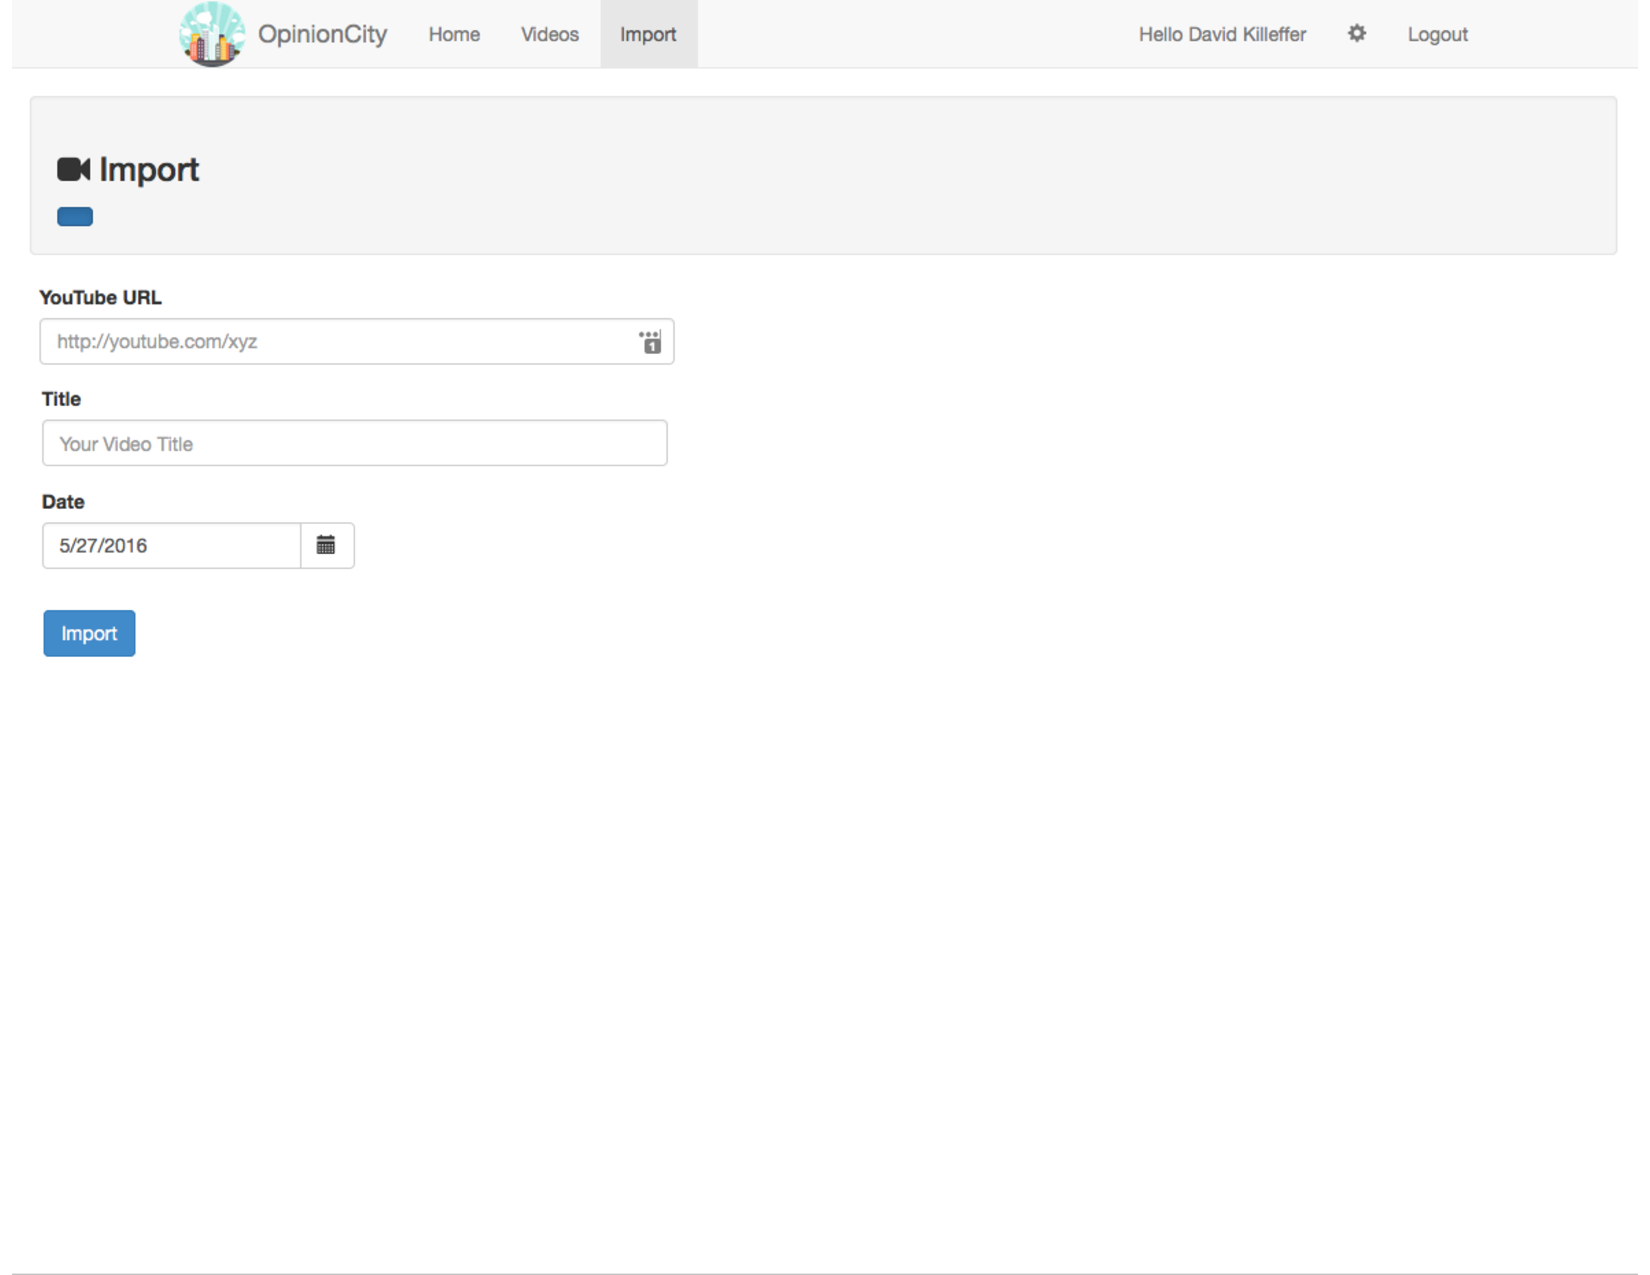
\includegraphics[width=1\textwidth]{gfx/opinion-city/import1.pdf}} \\
{\centering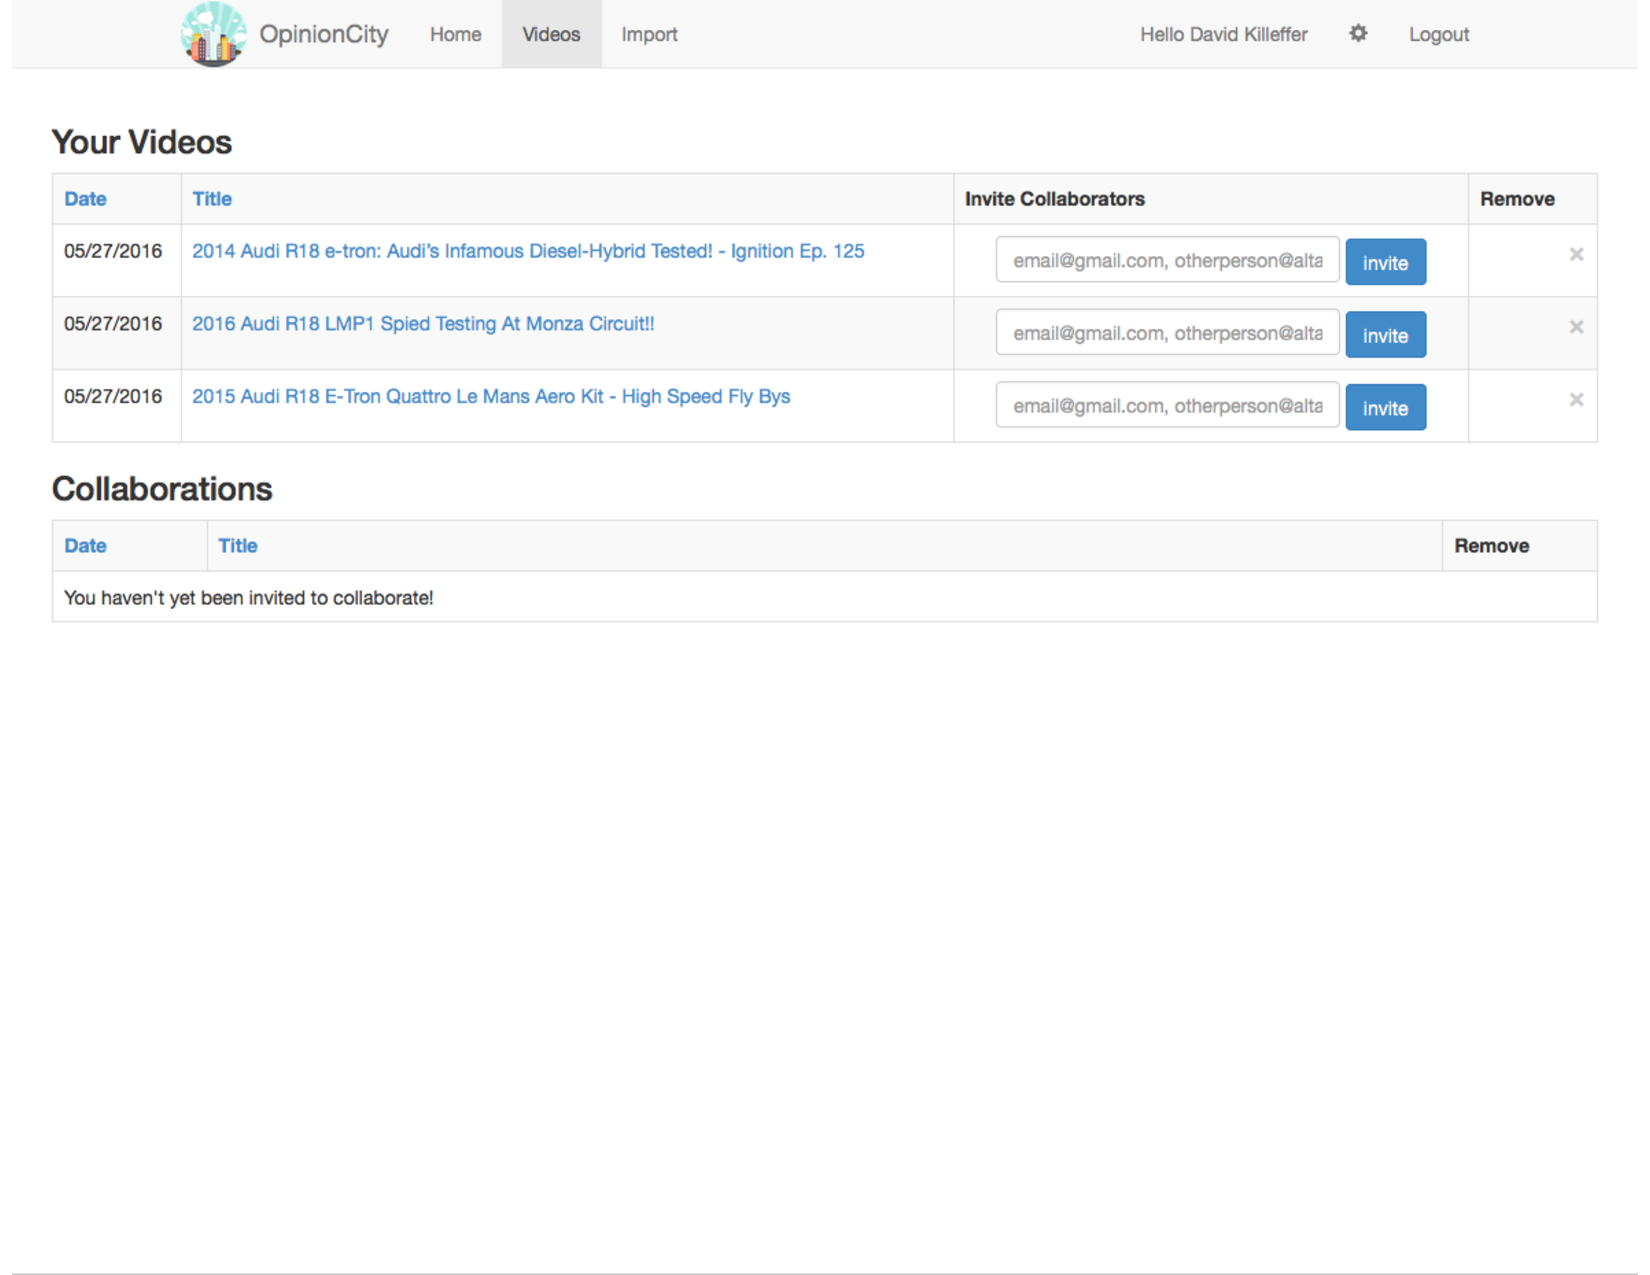
\includegraphics[width=1\textwidth]{gfx/opinion-city/videolist1.pdf}} \\
{\centering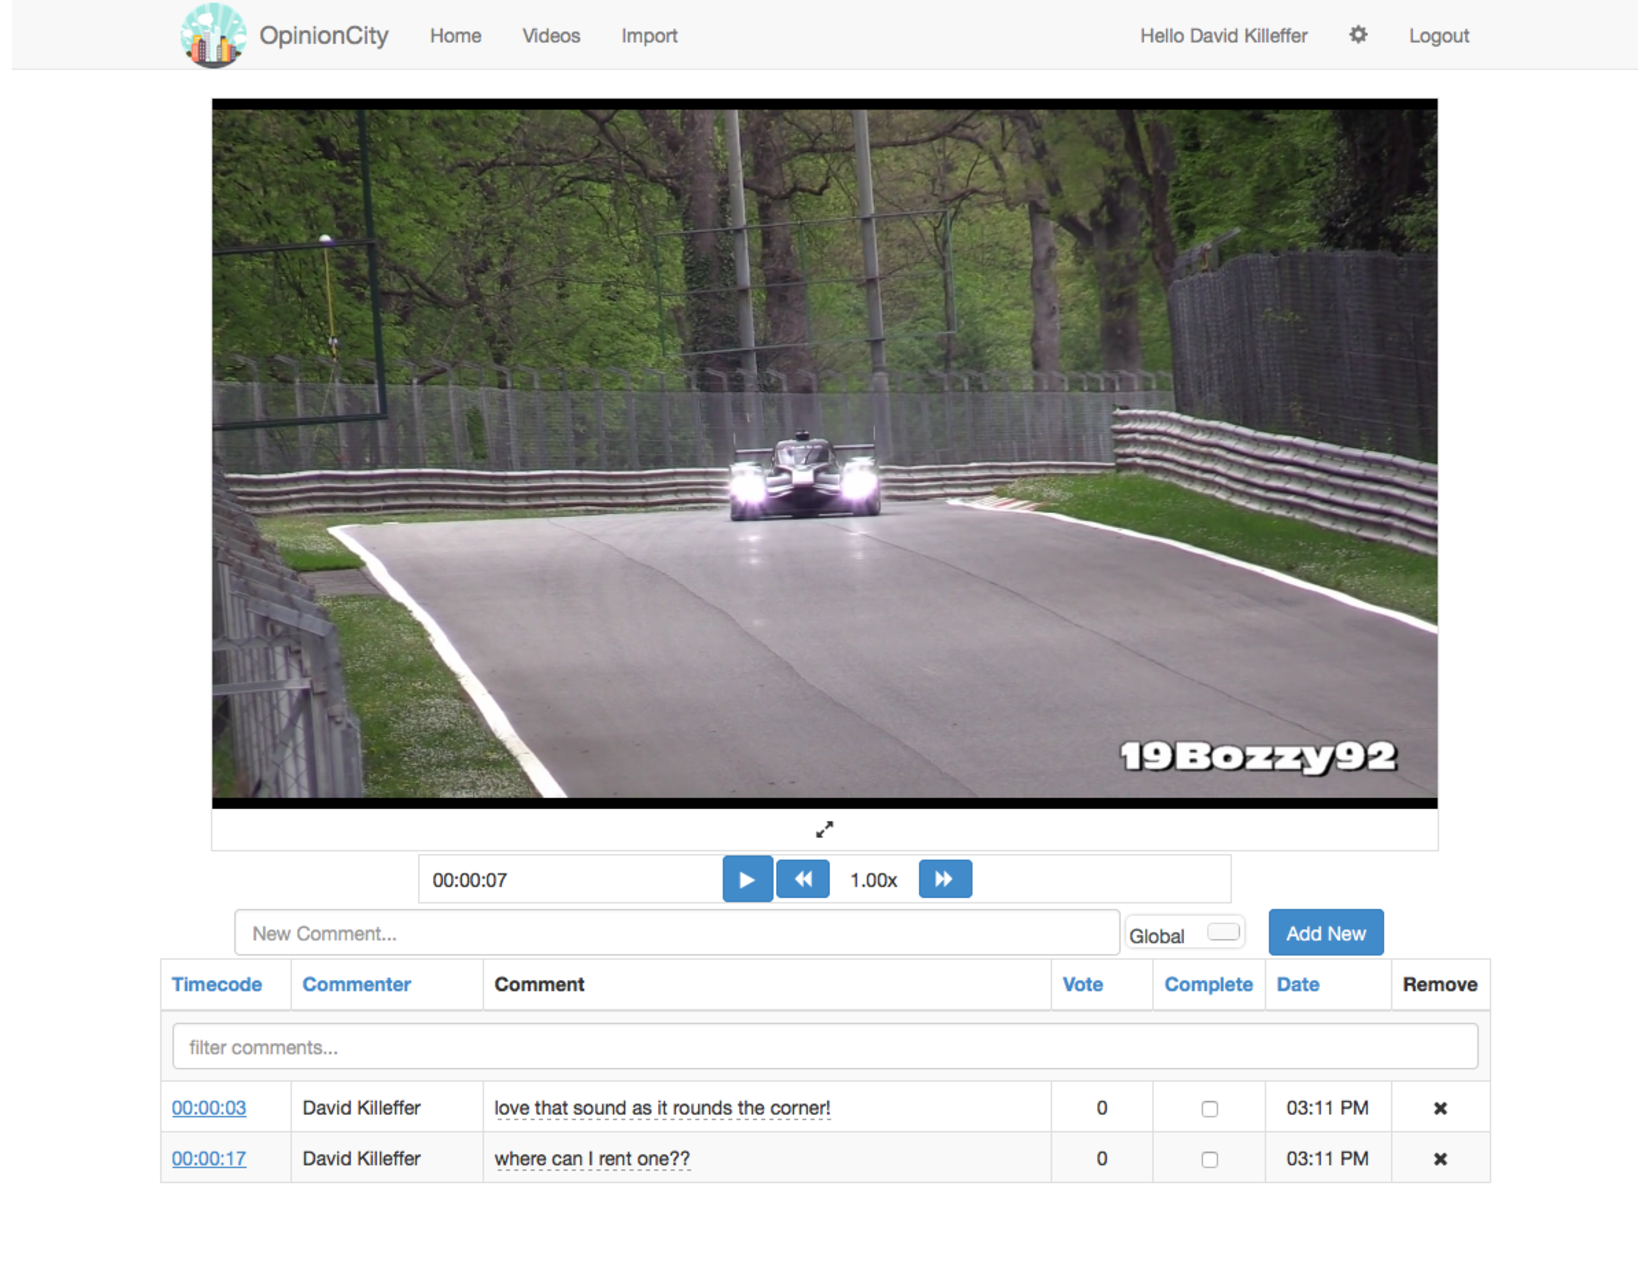
\includegraphics[width=1\textwidth]{gfx/opinion-city/car1.pdf}} \\
{\centering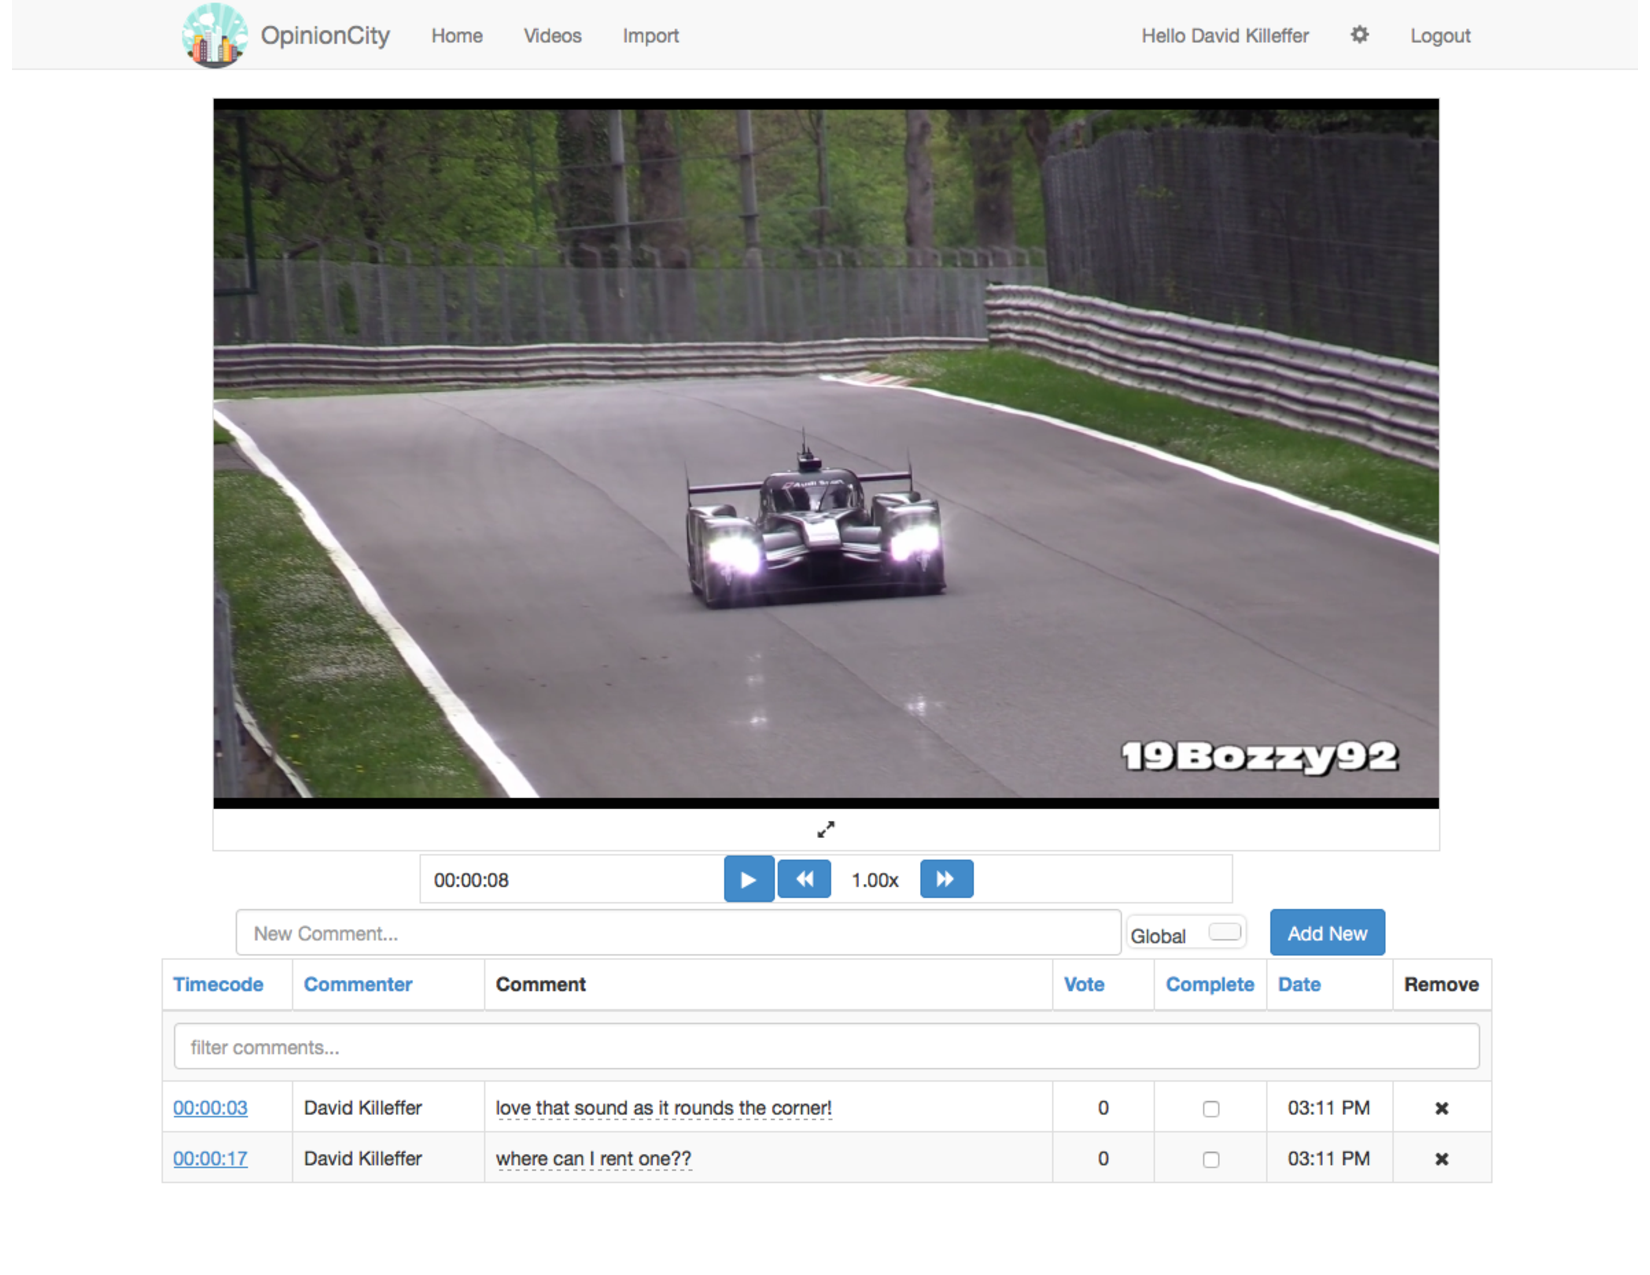
\includegraphics[width=1\textwidth]{gfx/opinion-city/car2.pdf}} \\


%	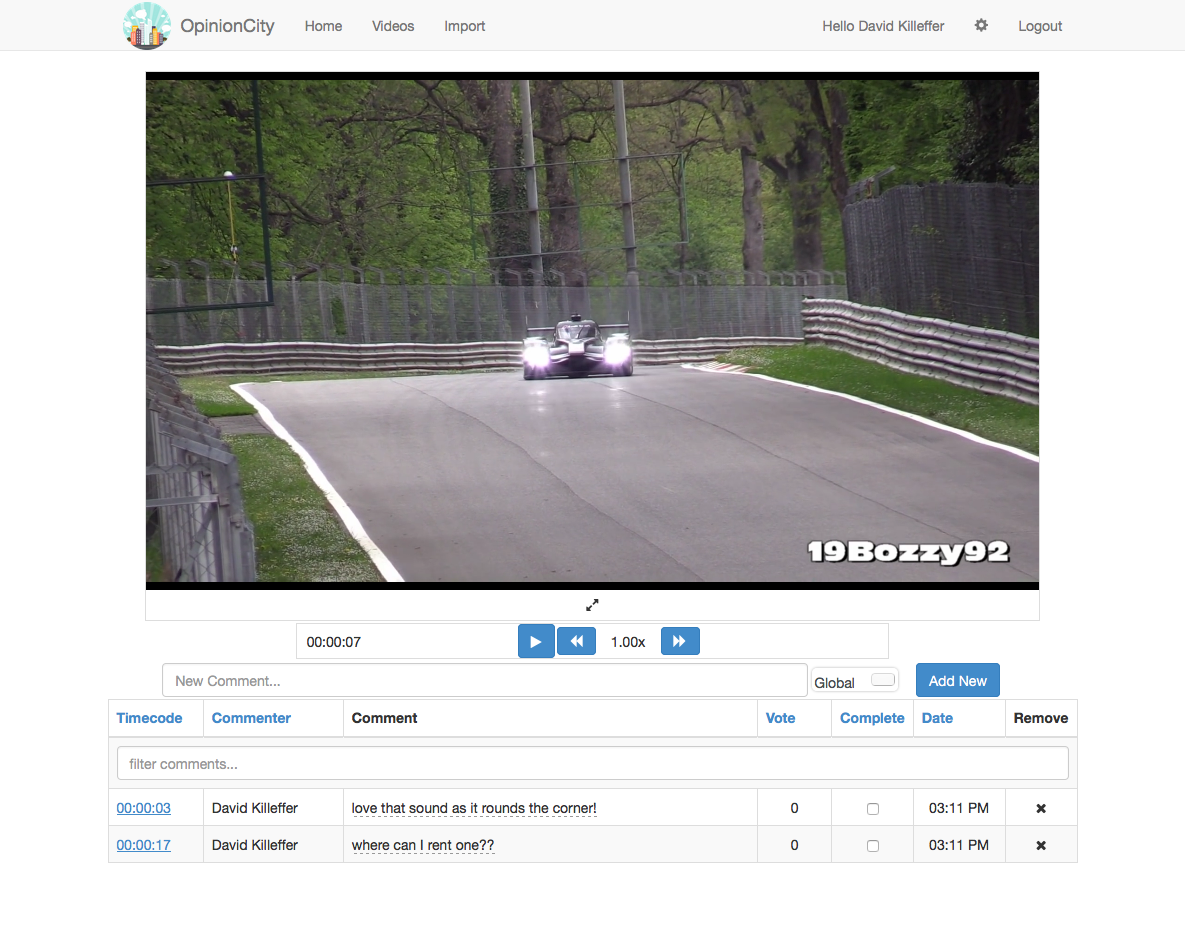
\includegraphics[width=18cm]{gfx/opinion-city/car1.png} \\[2mm]
%	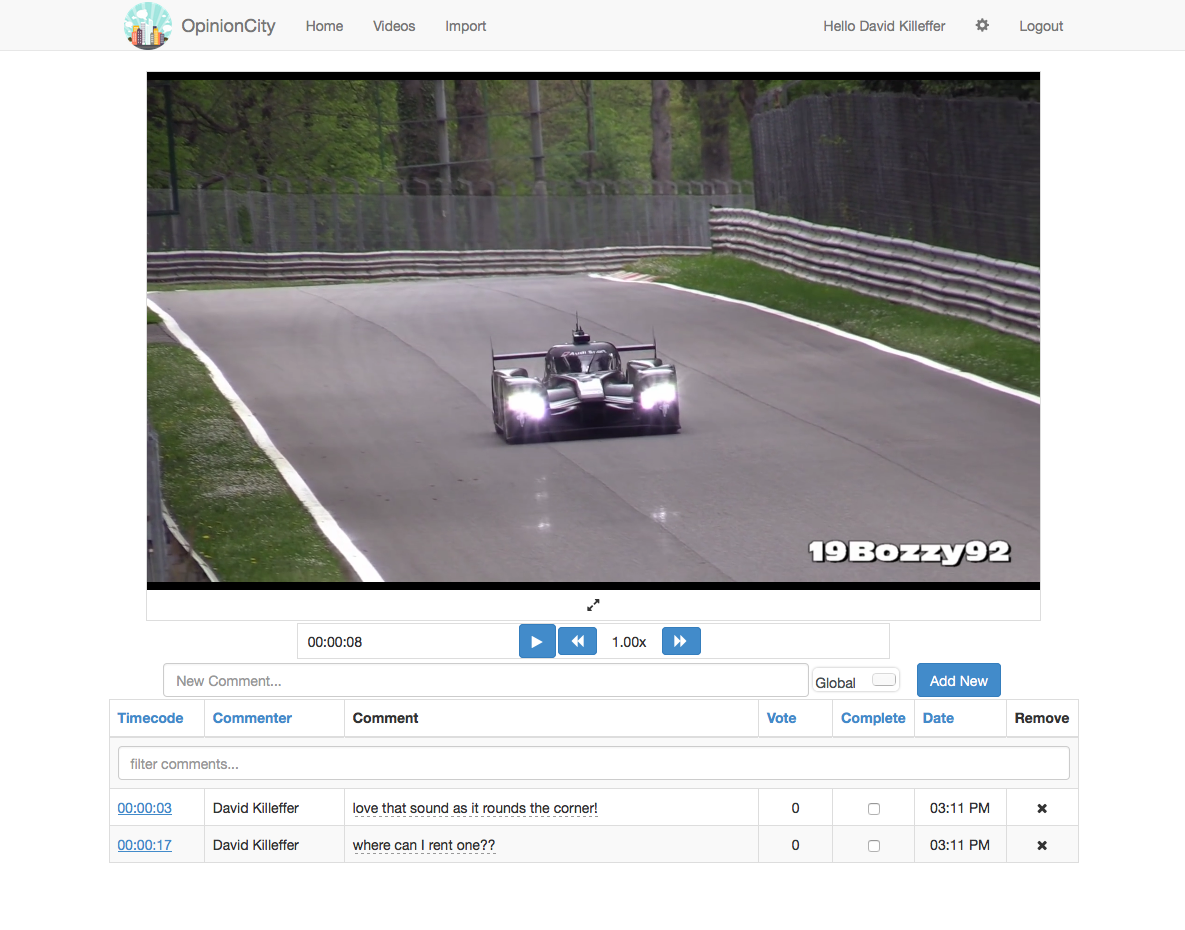
\includegraphics[width=18cm]{gfx/opinion-city/car2.png} \\[2mm]
%	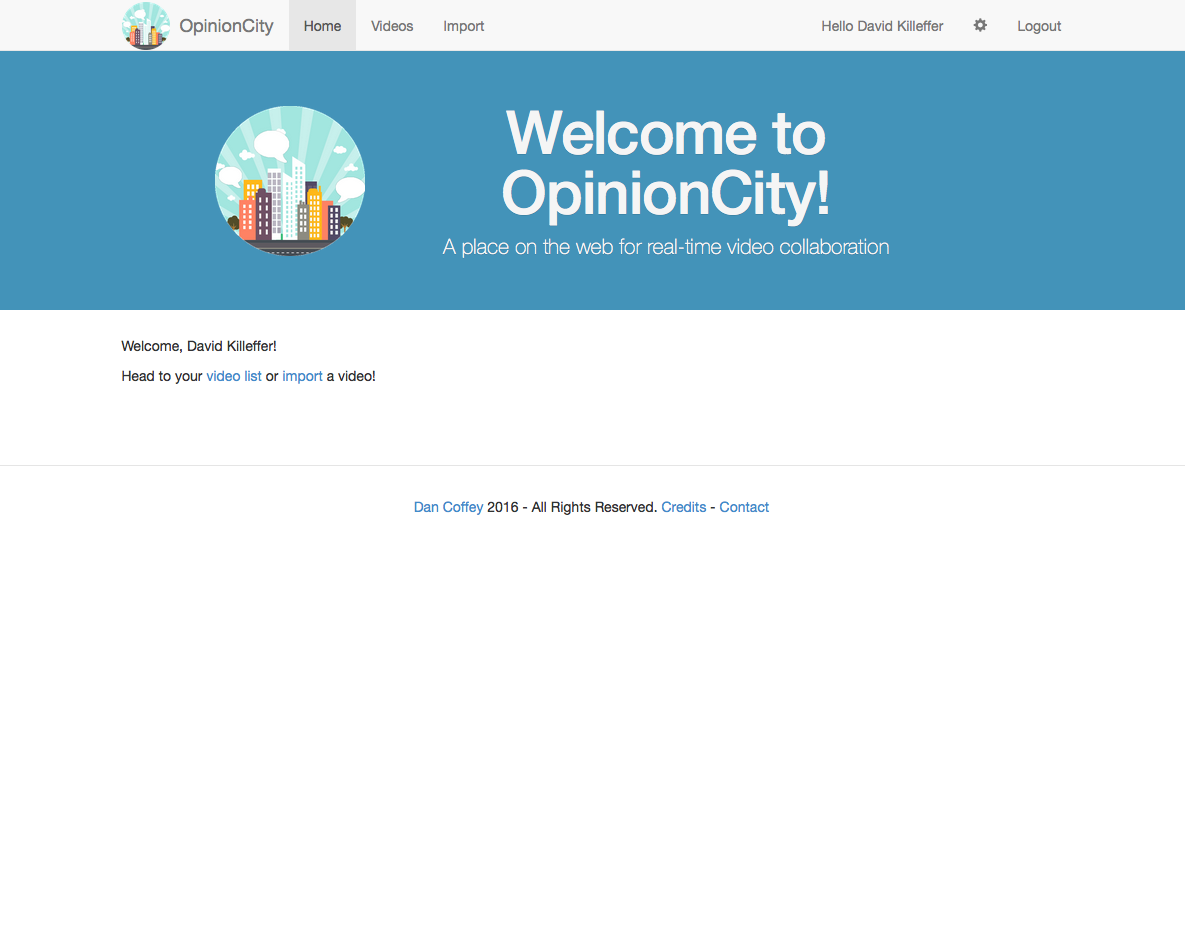
\includegraphics[width=18cm]{gfx/opinion-city/homepage1.png} \\[2mm]
%	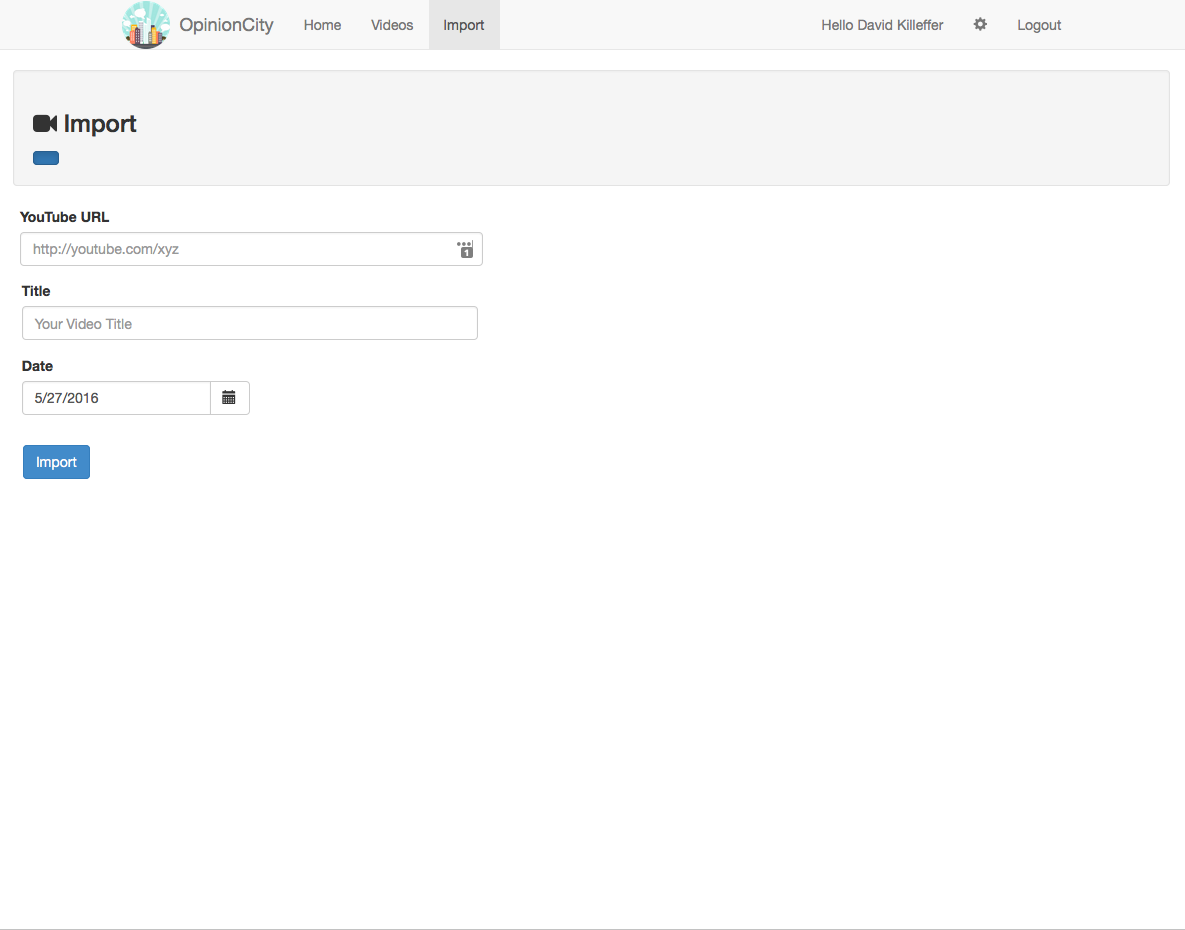
\includegraphics[width=18cm]{gfx/opinion-city/import1.png} \\[2mm]
%	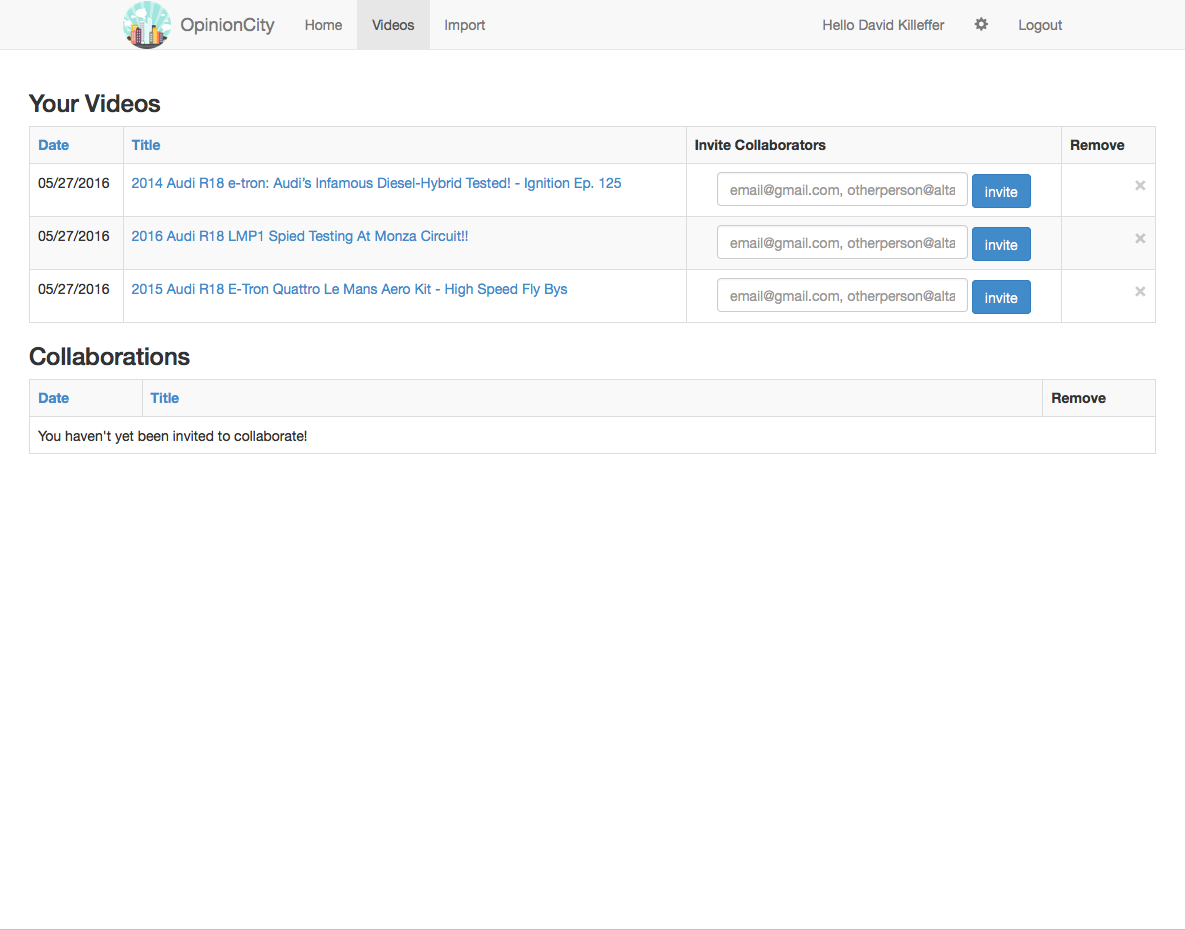
\includegraphics[width=18cm]{gfx/opinion-city/videolist1.png} \\[2mm]

%	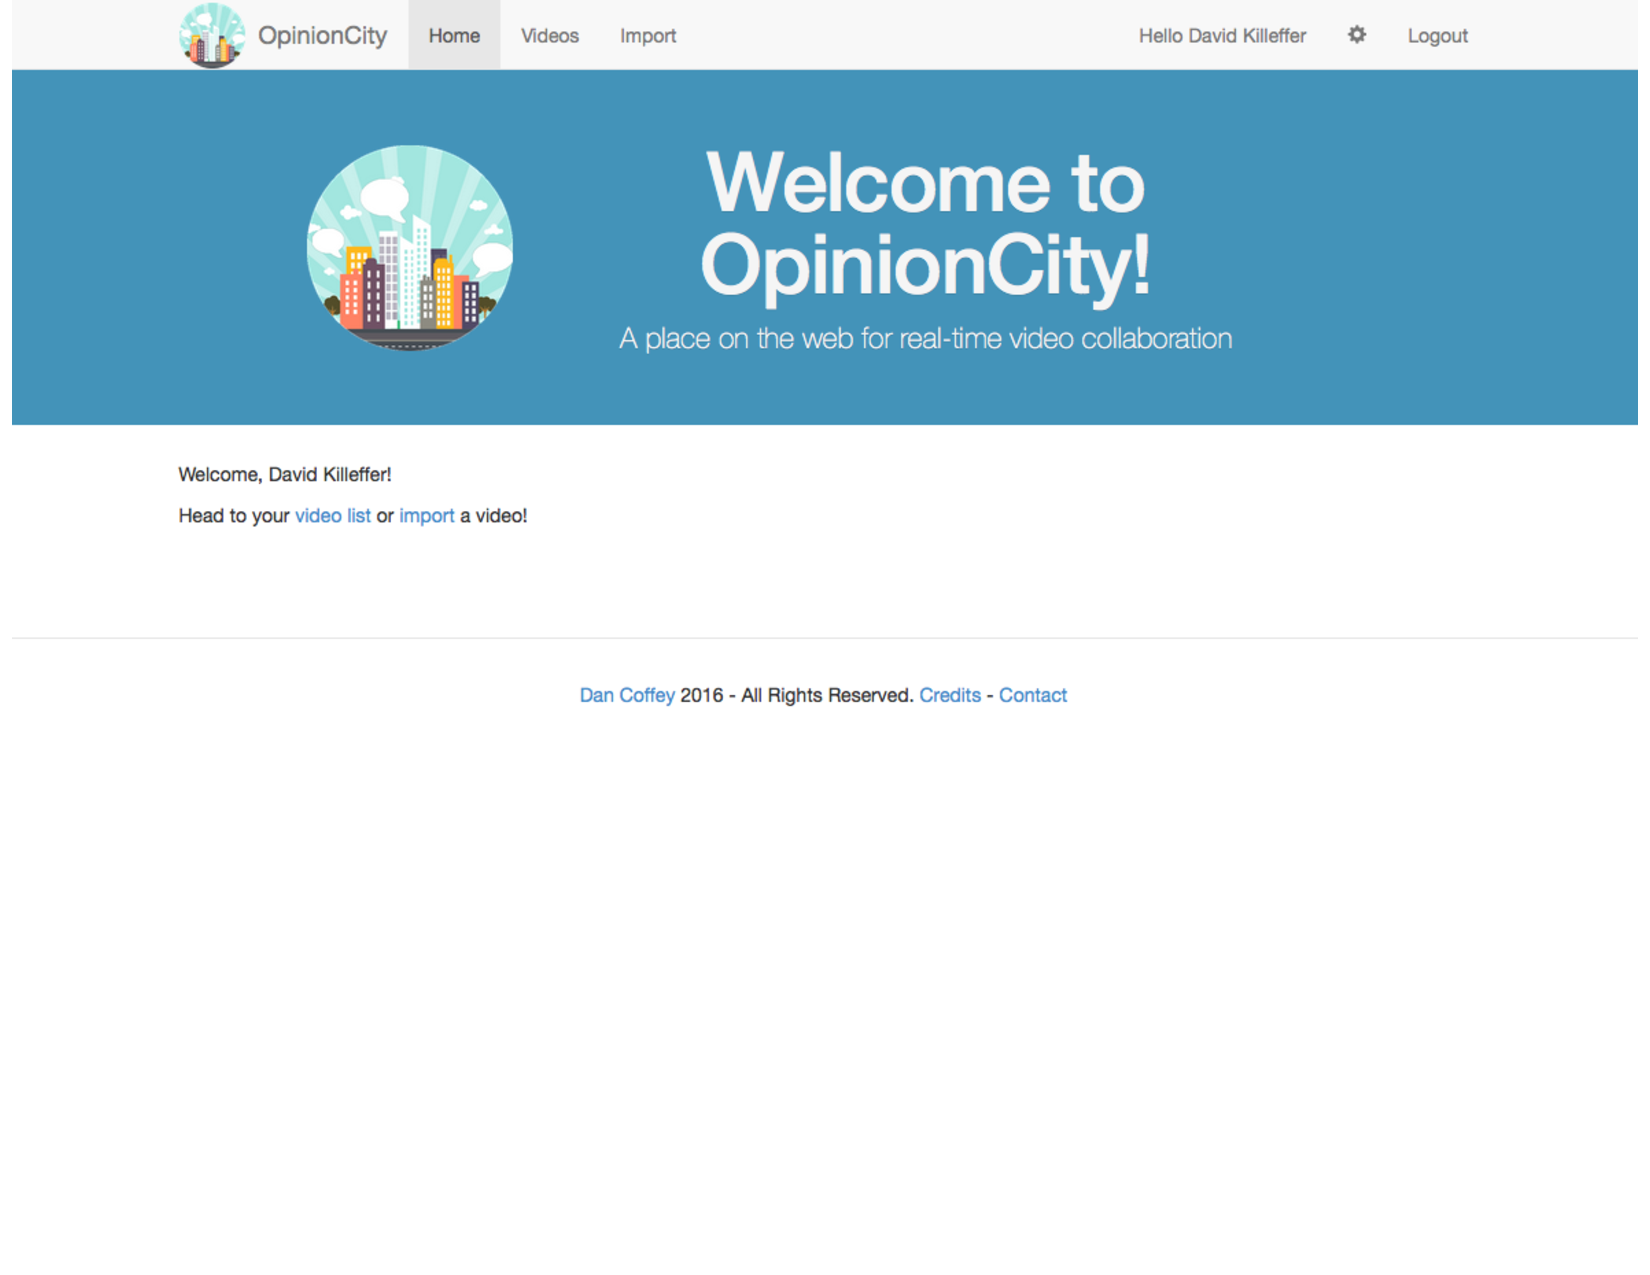
\includegraphics[width=6cm]{gfx/opinion-city/opinioncity-homepage1} \\[2mm]

%	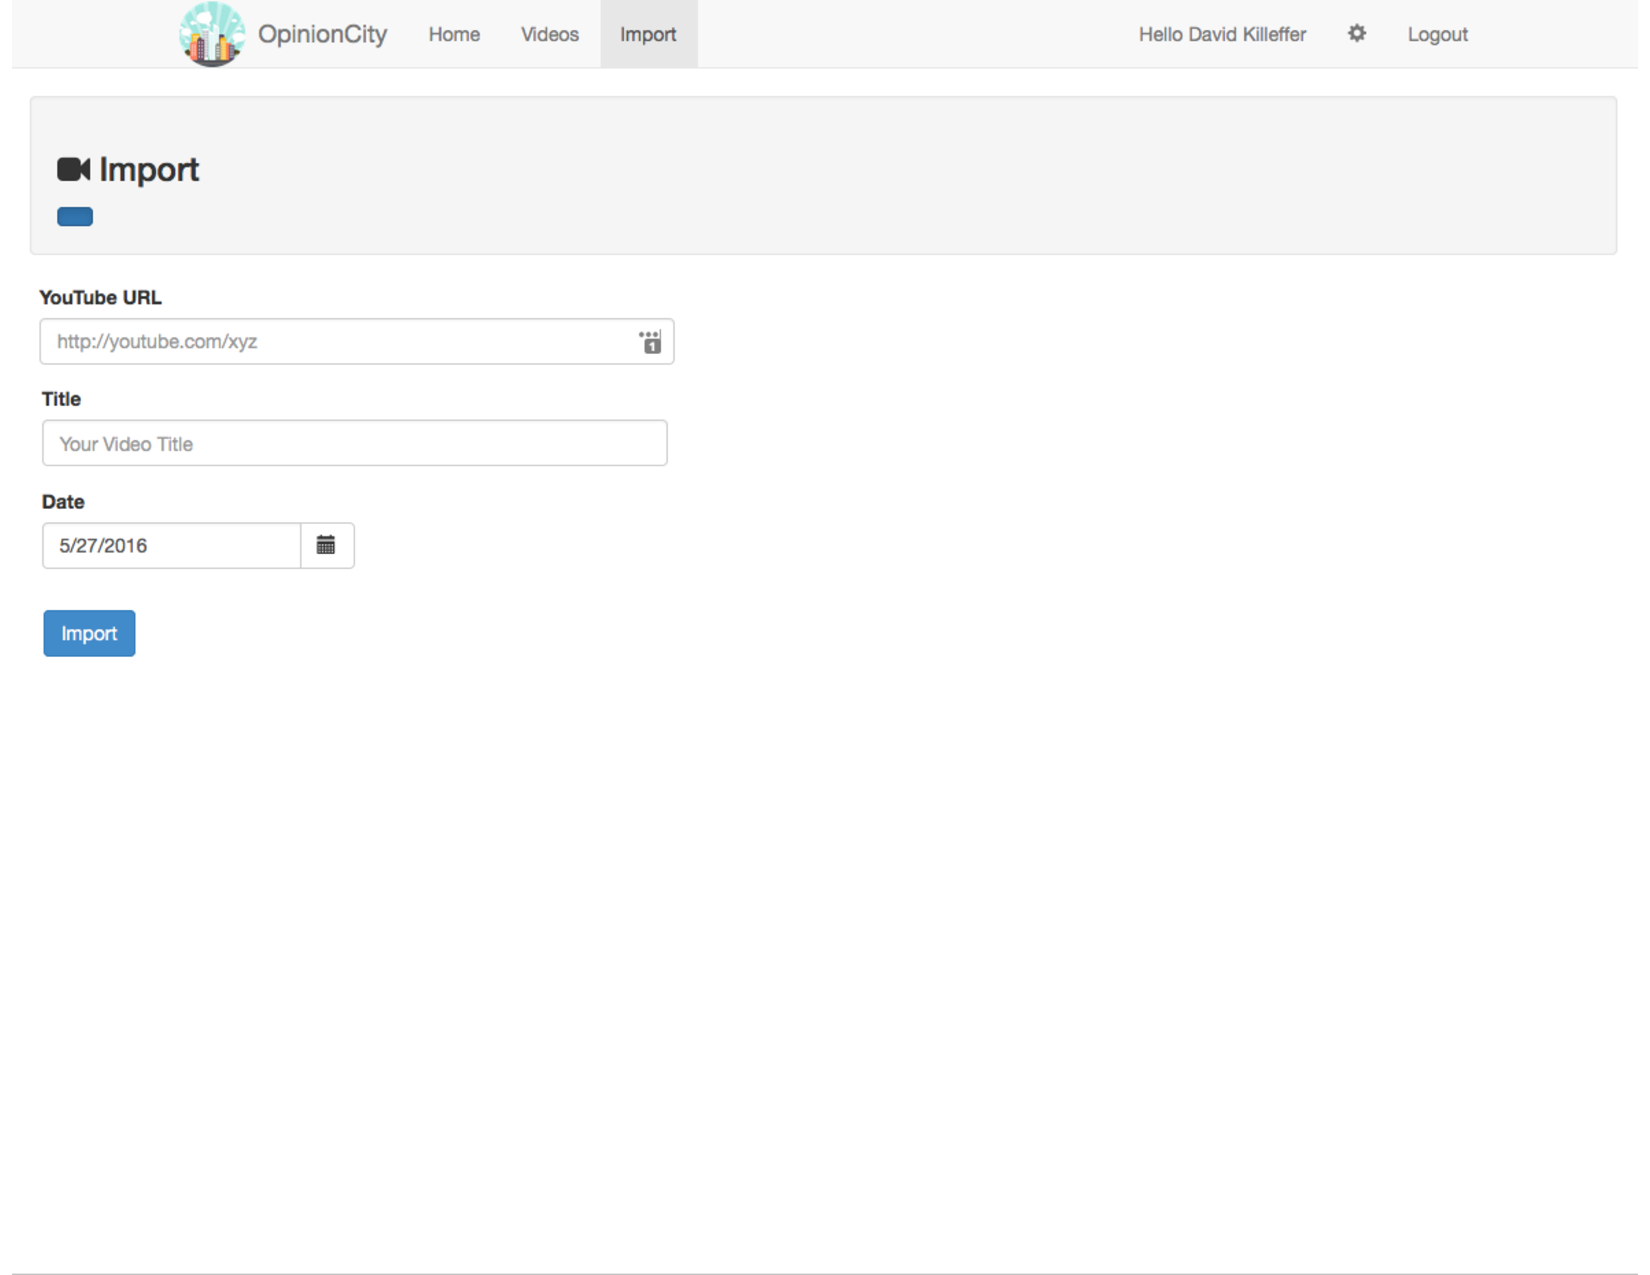
\includegraphics[width=6cm]{gfx/opinion-city/opinioncity-import1} \\[2mm]
%	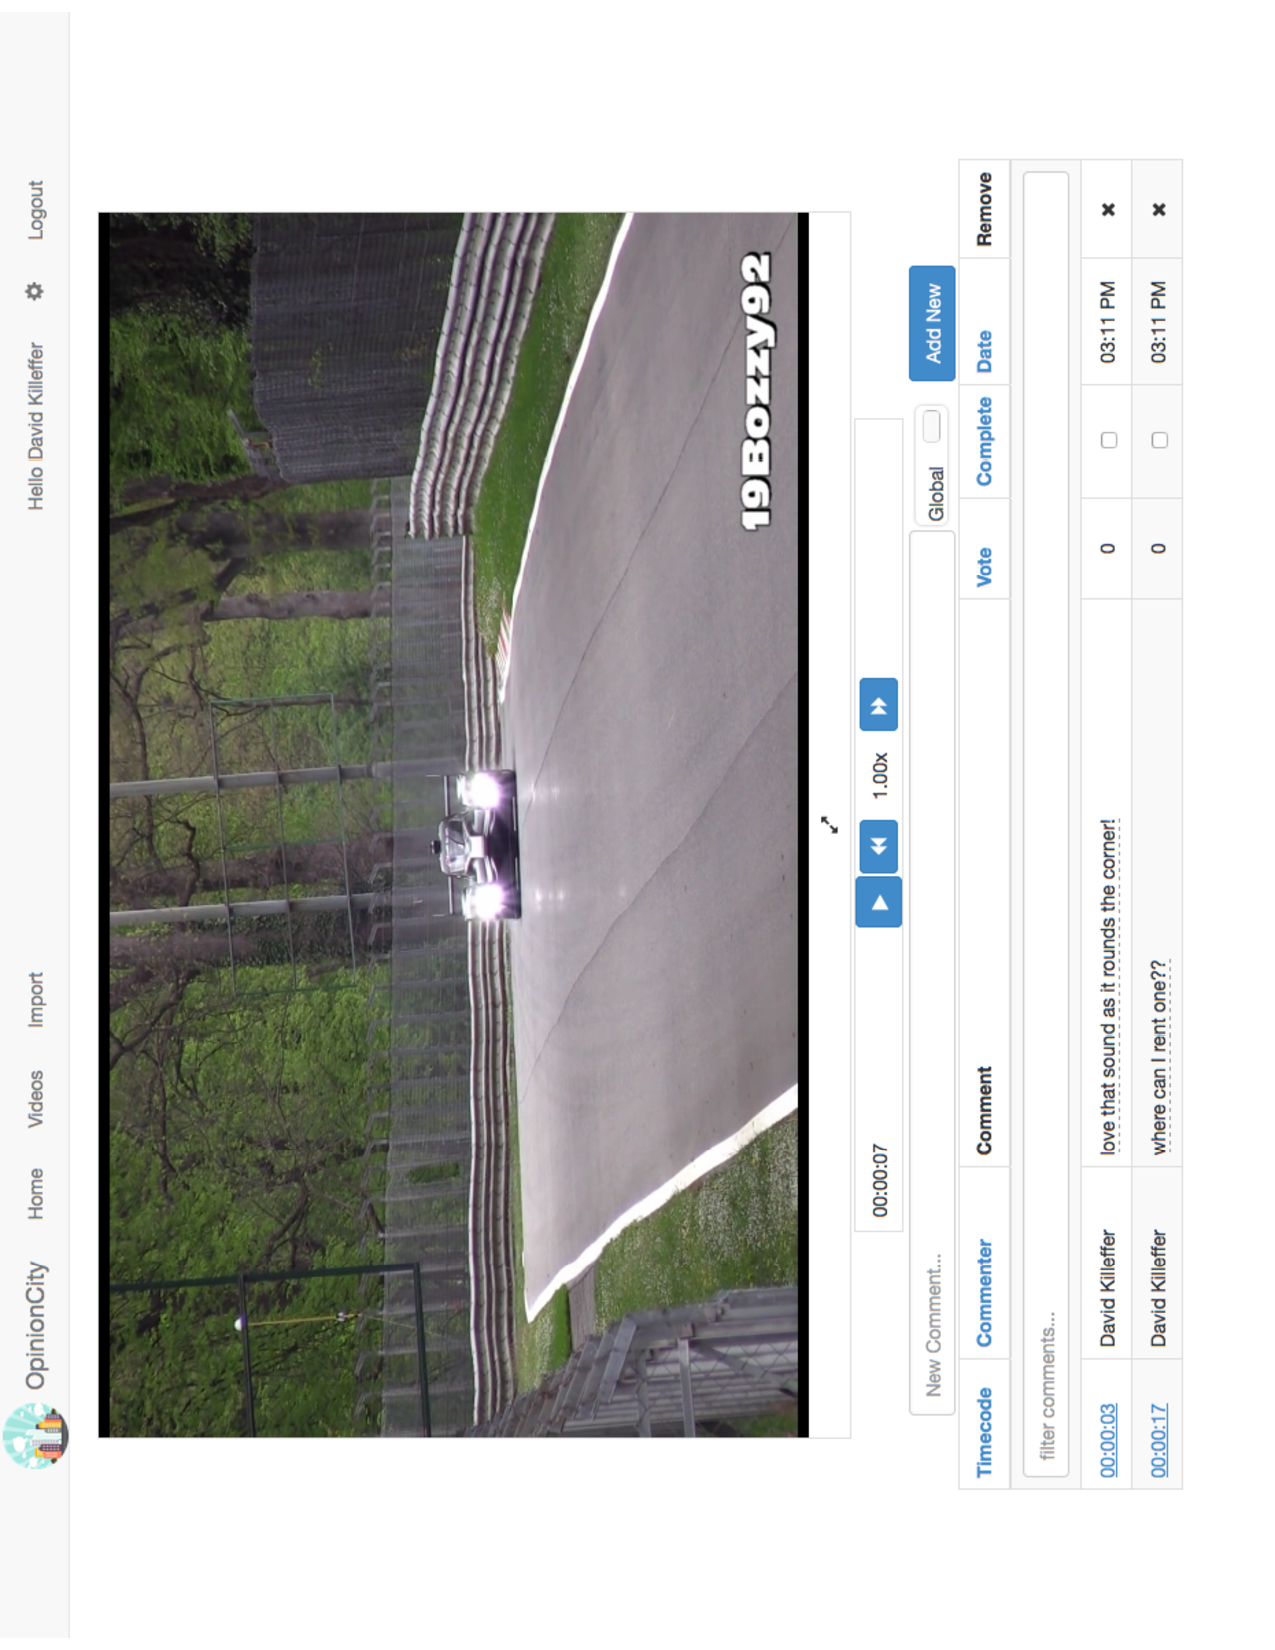
\includegraphics[width=6cm]{gfx/opinion-city/opinioncity-video1} \\[2mm]
%	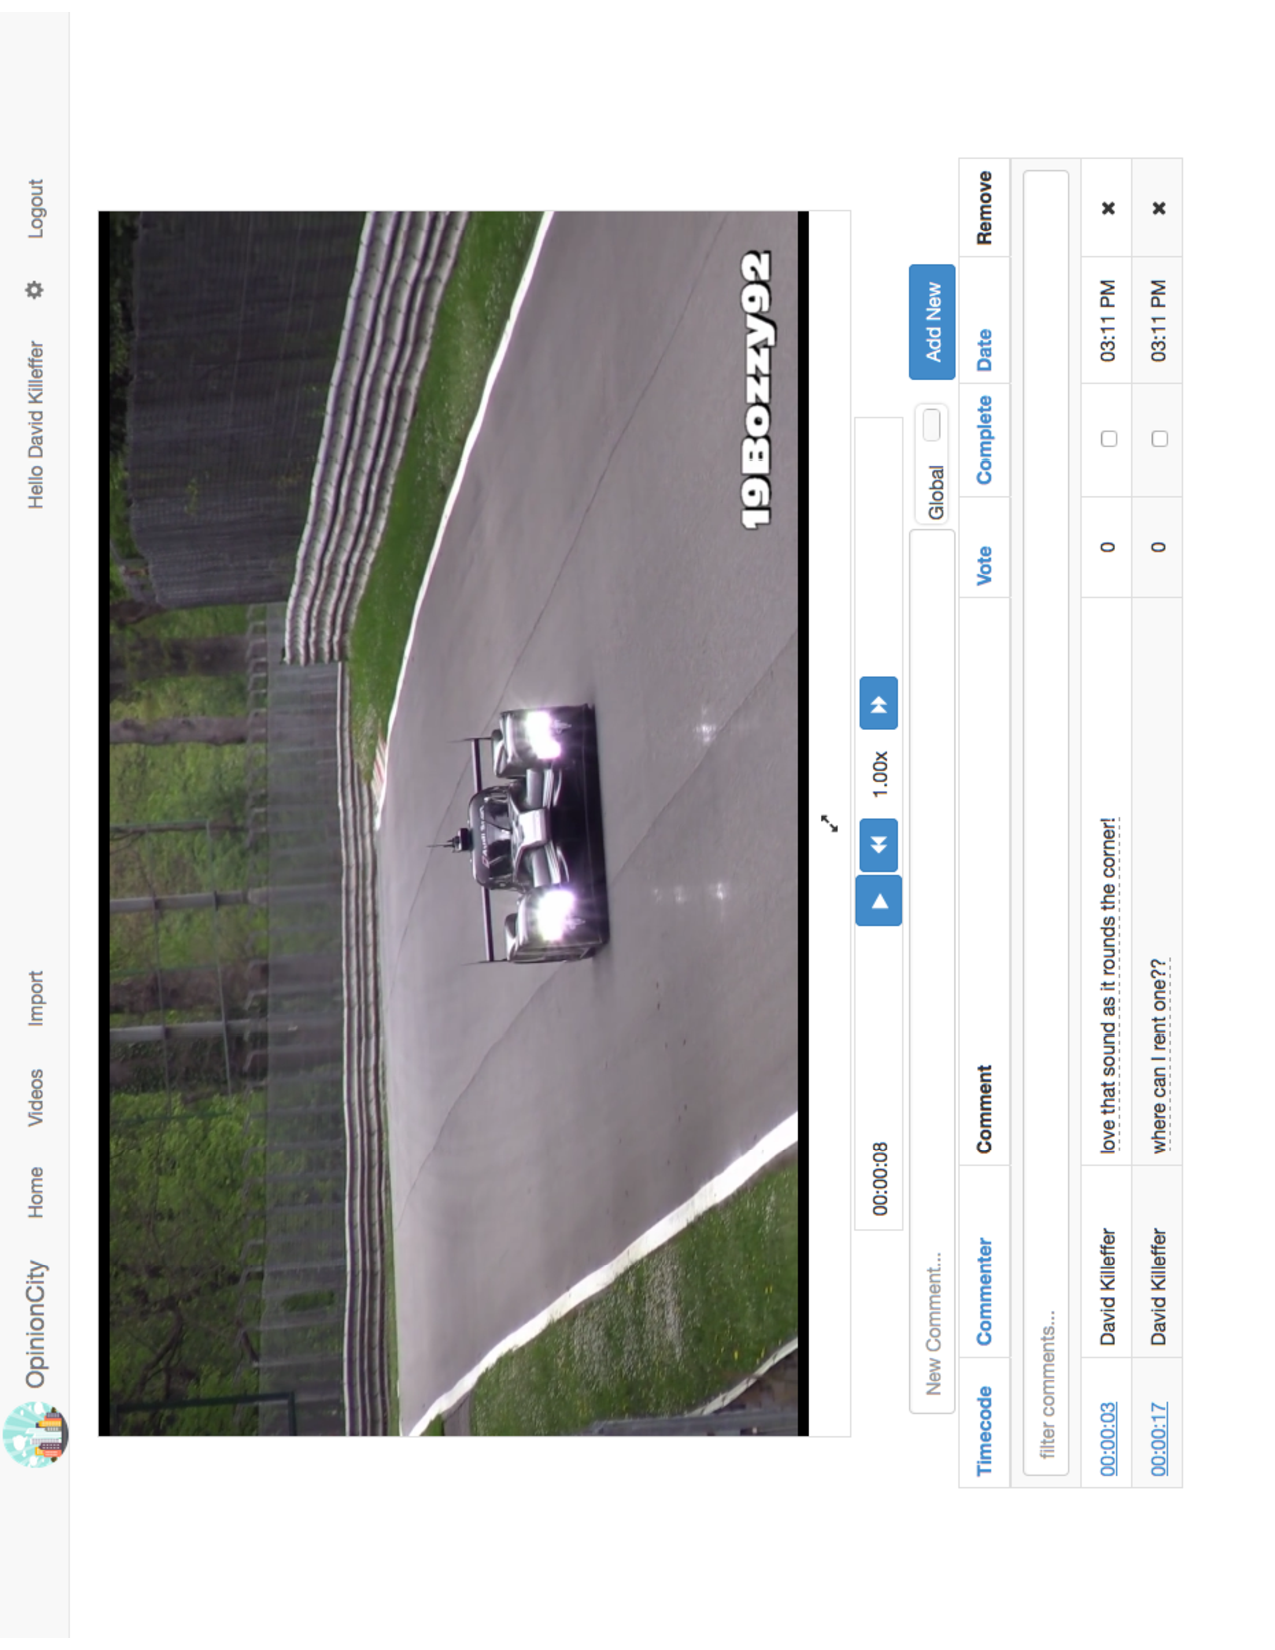
\includegraphics[width=6cm]{gfx/opinion-city/opinioncity-video2} \\[2mm]
%	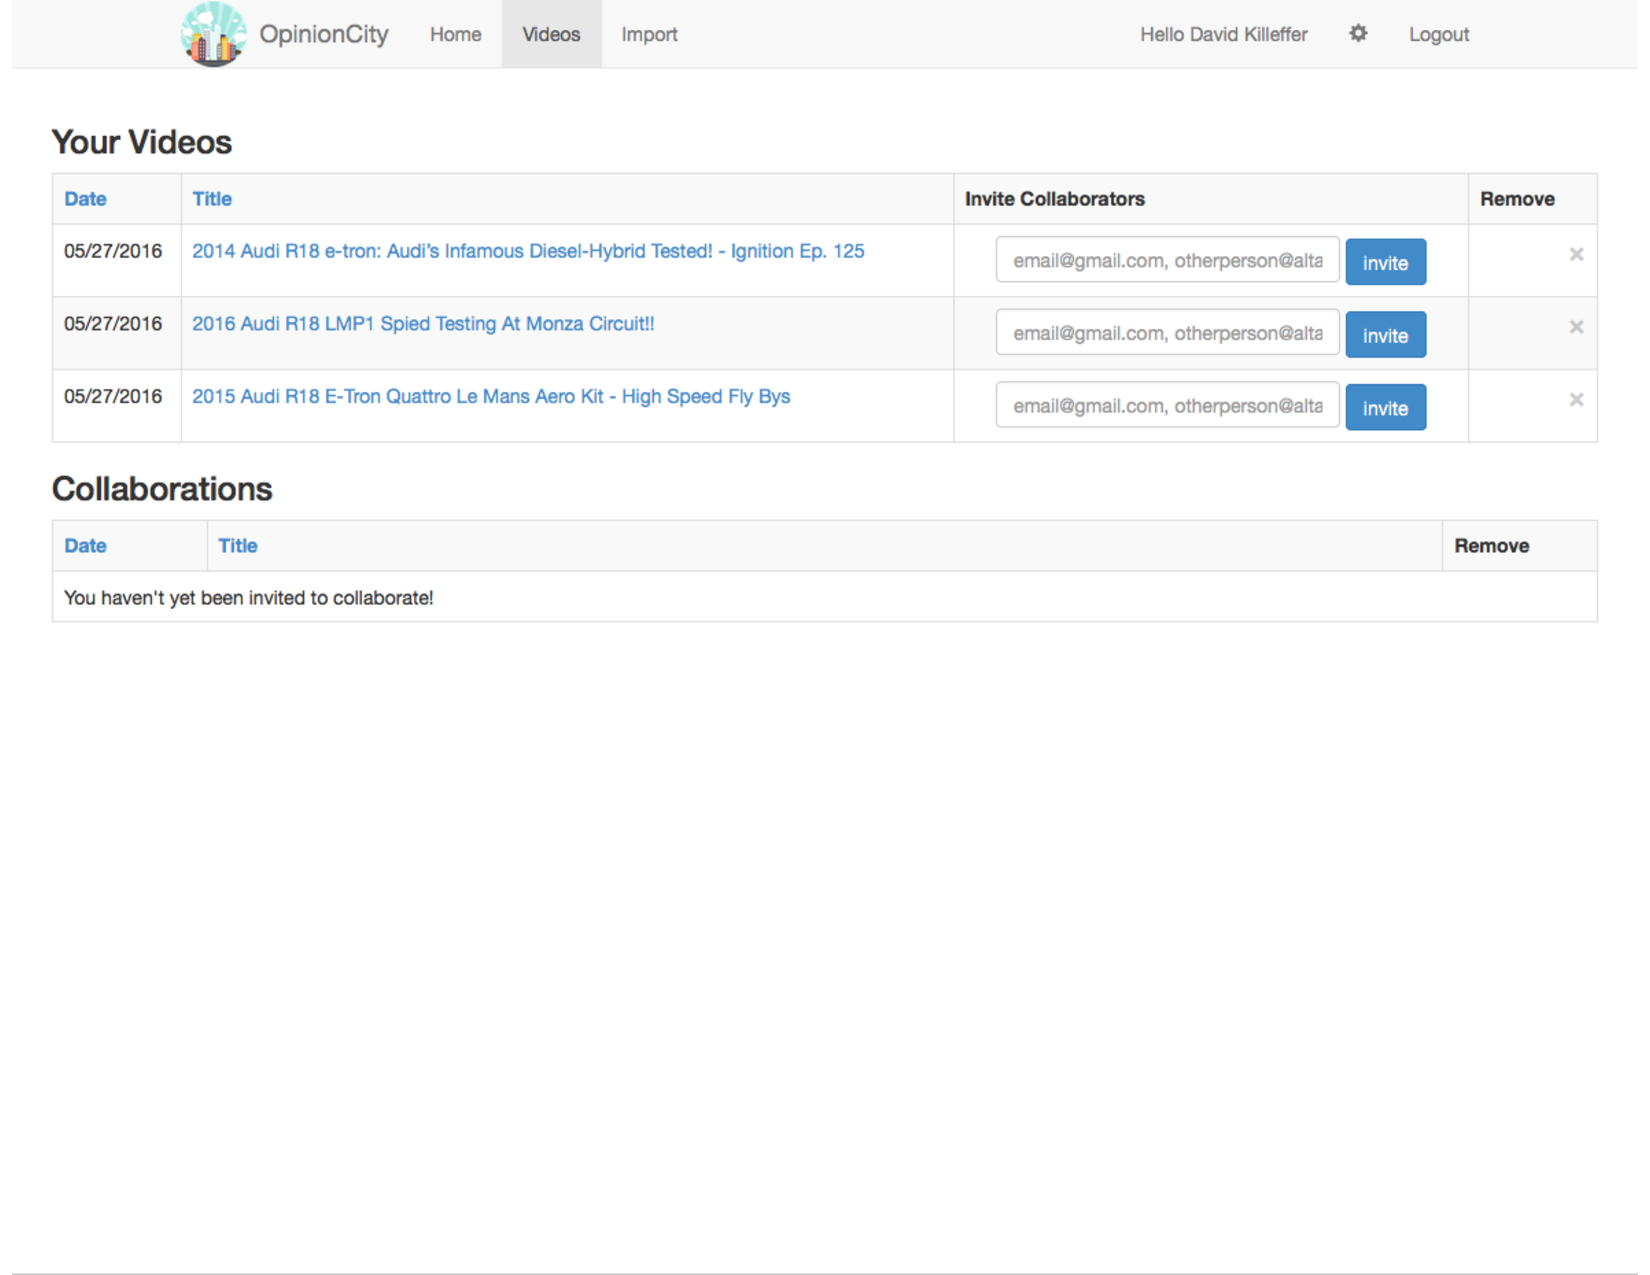
\includegraphics[width=6cm]{gfx/opinion-city/opinioncity-videolist1} \\[2mm]
%\end{center}



\item Phil's thesis
\end{enumerate}



\section{Prior Work Section 1}
\label{sec:priorwork:sec1}

%\Blindtext[2][2]

\section{Prior Work Section 2}
\label{sec:priorwork:sec2}

%\Blindtext[3][2]

\section{Prior Work Section 3}
\label{sec:priorwork:sec3}

%\Blindtext[4][2]

\section{Conclusion}
\label{sec:priorwork:conclusion}

%\Blindtext[2][1]
